\documentclass{MScthesisITEM}

% this package is just to generate text for demo-purposes
%\usepackage{blindtext}
\usepackage{float}

\usepackage{hyperref}
\usepackage{pdfpages}
\usepackage{tabulary}
%\usepackage[section]{minted}
%\usepackage{aeguill}
%\usepackage{placeins}
%\usepackage[T1]{fontenc}
%\usepackage{tabulary}

\showboxdepth=5
\showboxbreadth=5

\title{Learning Modeling Languages Using\newlinetitle Strategies from Gaming} % The title of your assignement; NB use \newlinetitle to start a newline
\author{\O yvin Richardsen} % Your firstname and lastname
\professor{Frank Alexander Kraemer, ITEM NTNU} % Affiliation = ITEM for instance
\supervisor{Frank Alexander Kraemer, ITEM NTNU}

%% Uncomment the following in case you want subfigures; note that there will be a warning for the caption package
%\let\subcaption\undefined
%\let\subfloat\undefined
%\usepackage[bf]{caption}
%\usepackage{subcaption}
%\captionsetup{compatibility=false}


\DeclareGraphicsExtensions{.pdf,.jpg,.png}
\graphicspath{{./img/}}

\loadglsentries{glossary}
\makeglossaries

\begin{document}
\selectlanguage{english}
\pagenumbering{roman}
\pagestyle{plain}

%% Only for the project
%\titleITEM

%% Only for the master's thesis; for the project report the description is taken from It's Learning and added by the department
\selectlanguage{english} % Change to 'norsk' if you are writing in Norwegian
%\chapter*{Problem Description}
When learning to use a software modeling language, people are usually directed towards the language's documentation, or ``language tutorials'' in the form of a set of instructions required to get started with the language. Most of the information about the language is generally delivered early in the process, requiring the developer to either understand (and remember) a lot of concepts at once, or to go back and search for the information when it's needed.

\noindent
On the contrary, many computer games come with no instructions at all, but rather start by guiding the player through a set of training levels. Each level introduces a new element, concept or strategy, and sometimes let the player experiment with the new concepts to solve more advanced problems.

\noindent
In this thesis, it will be examined to which degree this approach can be used for introducing and learning a new modeling language. Methods for creating more immersive tutorial experiences with required information delivered in-context will be explored and tested, using UML Activities and the Reactive Blocks tool as an example. The thesis will also explore whether the context of the tutorial matters, and if there are possible advantages gained by designing the tutorial experience itself as a game.

\noindent
\textbf{Assignment given:} \emph{Learning Modeling Languages Using Strategies From Gaming} \\
\textbf{Supervisor:} Frank Alexander Kraemer
\cleardoublepage

%% There must be an abstract in English, even though the main text is in Norwegian
\selectlanguage{english}
\chapter*{Abstract}

\cleardoublepage

%% Only for the master's thesis; if the main text is in English and you can write Norwegian, there must be an abstract in Norwegian as well.A
\selectlanguage{norsk}
Abstract nor: TODO
\cleardoublepage

\selectlanguage{english}% Change to 'norsk' if you are writing in Norwegian

\chapter*{Preface}

This thesis is submitted as the concluding part of my Master of Science degree in Communication Technology at the \gls{ntnu}. The supervisor for this thesis has been Associate Professor Frank A. Kraemer, and I would like to thank him for his help and guidance. I would also like to thank the people who helped me with the testing of my work.

\noindent
Trondheim, June 2014 \\
{\O}yvin Richardsen
\cleardoublepage

% similarly you may add a separate acknowledgments page

\tableofcontents*
\cleardoublepage

%% include if relevant
\listoffigures
\cleardoublepage

%% include if relevant
\listoftables
\cleardoublepage

%% include if relevant
%\listofalgorithms
%\addcontentsline{toc}{chapter}{List of Algorithms}
%\cleardoublepage


%% include if relevant
%\printglossary[title=List of Symbols, style=long]
%\cleardoublepage
%\glsaddall[]

%% include if relevant
\printglossary[title=List of Acronyms,type=\acronymtype] % prints just the list of acronyms
\cleardoublepage

\pagenumbering{arabic}
\pagestyle{ruled}
\chapter{Introduction}
\label{ch:intro}

\section{Problem Definition and Scope}
\label{sec:scope}


\subsection{Organization of the Report}
\cleardoublepage
\chapter{Background}
\label{ch:background}
This chapter contains the background material that serves as the basis for this thesis. The following sections are a mix of summarizations of other people's work, and some gathering and analysis of information done by me.


\section{Software Modeling and Modeling Languages}
\label{sec:software_modeling}
In the world of software development, potential problems and challenges that may arise when developing a product are plentiful.


\subsection{The Purpose of Software Modeling}


\subsection{Modeling Languages}


\subsection{Automatic Code Generation}


\section{Tutorials}
\label{sec:tutorials}
``A tutorial is a method of transferring knowledge and may be used as a part of a learning process. More interactive and specific than a book or a lecture, a tutorial seeks to teach by example and supply the information to complete a certain task.''~\cite{wiki:tutorial}

\noindent
Tutorials are often used to teach and introduce new concepts and topics to users who previously have little or no experience with it. Tutorials may be designed for learning a vast range of topics and concepts, such as:
\begin{itemize}
	\item Programming, or using specific programming or modeling languages.\footnote{\url{http://docs.oracle.com/javase/tutorial/}, \url{http://www.tutorialspoint.com/uml/}}
	\item Spoken languages.\footnote{\url{http://ielanguages.com/}}
	\item Software products.\footnote{\url{http://www.photoshoptutorials.ws/category/photoshop-tutorials/}}
	\item Video games (such tutorials are usually presented inside the game itself)
	\item Real-life skills, like photography.\footnote{\url{http://photography.tutsplus.com/}}
	\item Human sciences.\footnote{\url{http://anthro.palomar.edu/tutorials/}}
\end{itemize}

\noindent
The above list is in no way exhaustive, but meant to offer some examples of the numerous and diverse topics that may be introduced with the help of a tutorial.

\noindent
Additionally, tutorials come in many forms. The most common form of tutorial is likely the text-based tutorial, often supplemented by illustrations and pictures, but tutorials also come in the form of videos, animations, audio, or in the case of many video games, an interactive experience combining any or all of these.

\subsection{The Structure of a Tutorial}
\label{sec:tutorial_structure}
Tutorials for different types of topics are generally structured in a way the author believes will provide a good introduction for the given topic, starting with the necessary basic information, and then building on this to learn more advanced concepts. Depending on both the topic and the author, this may result in very different structures.

\noindent
Looking at some of the examples from Sect.~\ref{sec:tutorials}, we see that while the Java tutorials provide stepwise instructions for reaching a specific goal, the spoken language tutorials serve as more of a lookup reference for the most basic concepts within the language. The spoken language tutorials are actually in some ways similar to the separate Java API documentation.\footnote{\url{http://docs.oracle.com/javase/8/docs/api/index.html}}

\noindent
While there are differences in how tutorials for various topics are made, we may infer some general patterns and elements present in a wide range of different tutorials.

\begin{itemize}
	\item Basic and/or advanced information about the topic, depending on the scope of the tutorial. Often presented in a stepwise manner, starting from the most basic and moving on to the more advanced.
	\item Examples on how to use the information provided in specific cases or contexts.
	\item Exercises where the reader must try to use the concepts introduced in a specific context.
	\item Illustrations, figures, or animations, providing the reader with additional examples, information about concepts, or desired results from exercises.
	\item Some kind of motivation for learning about the topic, often as part the tutorial introduction.
\end{itemize}

\noindent
How these patterns and elements are presented depends on the form of the tutorial.

\subsection{The Characteristics of a Tutorial}
\label{sec:tutorial_characteristics}


\subsection{What Makes a Tutorial Good?}


\section{Tutorials for Programming and Software Modeling}
\label{sec:programming_tutorials}
In order to teach potential users to use a specific programming language, paradigm, protocol or modeling language (from now on referred to simply as a \emph{topic}), various additional tools or sources of information may be provided. Generally, some form of formal documentation or specification of the language or protocol is considered mandatory, and serves as the \emph{definitive} source of information. Additionally, various tutorials and exercises are often created in order to provide a better introduction to the topic, decreasing the threshold for learning this topic.

\subsection{Documentation}
While a topic's documentation often serves as its primary source of information, such formal documents are not necessarily the best source of information when \emph{learning} about the given topic. Often it is not intended as a learning resource, but rather as a formal reference for users already familiar with the topic. In the documentation, the topic is generally presented in a structured way with respect to its various aspects, so that it is easy for someone already familiar with the topic to find the required information.

\noindent
A good example of this is the \gls{uml} specification.\footnote{\url{http://www.omg.org/spec/UML/2.4.1/}} While the specification offers detailed information about every aspect of \gls{uml} in a way that suits an experienced user, it is likely confusing and not particularly helpful for a user with no previous experience or knowledge about \gls{uml}. Using this specification as a starting point for learning \gls{uml} is likely to require a lot of effort from the user. In the worst case, the user may not even learn all the concepts properly, despite the provided information being very specific and accurate.

\noindent
More importantly, the user may not learn how to properly apply the learned concepts to a given situation. In many cases, 


\subsection{Advantages and Challenges}




\section{Game-based learning}
\label{sec:game_based_learning}

\subsection{Gamification}


\subsection{Learning Inside the Game}


\subsection{Applying Acquired Knowledge and Skills in the Game}




\section{Tutorials in Games}
\label{sec:tutorials_in_games}


\subsection{Purpose}

\subsection{Tutorial Characteristics and Their Importance}

presence, context-sensitivity, freedom, availability of help-on-demand





\cleardoublepage
\chapter{Analysis of Related Work}
\label{ch:related_work}
This chapter outlines previous work by other researchers that is relevant to this thesis, supplementing the background information provided in Ch.~\ref{ch:background}. A lot of work and research has been and is being done in the field of learning with games and game-like approaches, but for practical reasons (there is a lot of material) this chapter only summarizes what I've found to be most relevant. This primarily includes work on tutorial design and teaching computer-related tasks through games, but some other work is also included to add perspective.

\section{Tutorial Design}
\label{sec:tutorial_design_related}
Tutorials, as described in Sect.~\ref{sec:tutorials}, are widely used to teach users how to work with software products, among other things. With the tutorial, the creators aim to teach users how to perform various tasks with their tool, preferably in a \textbf{quick}, \textbf{intuitive}, \textbf{memorable}, and \textbf{error-free} way. Unfortunately, not all tutorial designs succeed in fulfilling all of these goals, but many efforts have been made to explore different approaches and improve on the standard tutorial design. Some of these are briefly described in the following sections.

\subsection{Stencils-Based Tutorials}
\label{sec:stencils}
The authors of the paper \emph{Stencils-Based Tutorials: Design and Evaluation}~\cite{kelleher:stencils} identify some problems with traditional tutorials: users may miss steps or perform actions that were not intended, and it is often difficult to find the components described in the tutorial.

\noindent
In their work, the authors introduce \emph{Stencils}, which is an alternative way of presenting a tutorial by adding a translucent colored interface layer on top of the original \gls{ui}, with holes highlighting the relevant elements, as seen in Fig.~\ref{fig:stencils}. Additionally, tutorial information is displayed on this layer in the form of sticky notes.

\begin{figure}[htp]
	\centering
	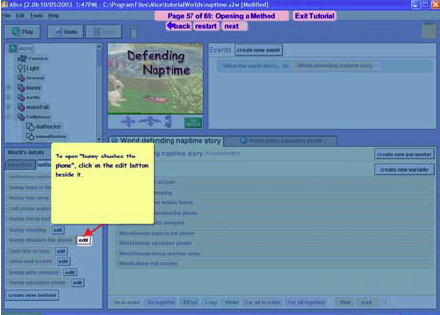
\includegraphics[width=0.8\textwidth]{stencils}
	\caption[\emph{Stencils} example]{An example of highlighting relevant \gls{ui} elements with \emph{Stencils} through holes in the colored layer. Tutorial information is added with the yellow sticky note. \emph{Image source:~\cite{kelleher:stencils}}}
	\label{fig:stencils}
\end{figure}

\noindent
With the results of a user study, the authors show that with a \emph{Stencils}-based tutorial, users were able to complete tutorials faster, with fewer errors and less human assistance. They also note that their tutorial approach can likely be improved by decreasing the level of assistance depending on the users familiarity with the system. A need for tutorial tasks that are directly relevant to the users, as opposed to ``artificial'' tutorial exercises, is also mentioned.


\subsection{DocWizards}
\label{sec:docwizards}
The authors of the paper \emph{DocWizards: A System for Authoring Follow-me Documentation Wizards}~\cite{bergman:docwizards} identify that there are some problems with teaching people to use software (\emph{computer-based procedures}) through documentation alone. Users must find \gls{ui} elements based on documentation descriptions on their own, understand and handle conditional branches, and at the same time keep track of where they are in the process.

\noindent
In their work, they propose the use of a tutorial-like documentation process called \emph{follow-me documentation wizards}, an approach that combines the advantages of conventional wizards and documentation. With their approach, processes are automatically captured from demonstrations made by expert users, and made available to new users in the form of highlighting both text from the documentation (see Fig.~\ref{fig:docwizards}) as well as UI elements for each step.

\begin{figure}[htp]
	\centering
	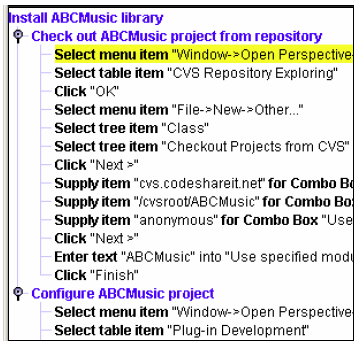
\includegraphics[width=0.6\textwidth]{docwizards}
	\caption[\emph{DocWizards} example]{An example of stepwise instructions in \emph{DocWizards}. The current step is highlighted in yellow. \emph{Image source:~\cite{bergman:docwizards}}}
	\label{fig:docwizards}
\end{figure}

\noindent
TODO: rewrite
Finally, a user study is conducted by the authors to evaluate their system, yielding positive results. The usefulness of the \emph{DocWizards} approach has also been verified in a separate study~\cite{gweon:evaluating_docwizards}.

\subsection{Graphstract}
\label{sec:graphstract}
The authors of the paper \emph{Graphstract: Minimal Graphical Help for Computers}~\cite{huang:graphstract} identify problems with the commonly used approach of providing only a textual explanations in software tutorials and help. Users are unlikely to read these explanations carefully enough, if at all. Simply adding screenshots of the \gls{ui} is not an adequate solution, since these usually add far more information than necessary, and thus increase the perceived size and complexity of the explanation. Problems with animation and video are also identified, such as making it difficult for the user to move at their own pace.

\noindent
Instead of relying on text-only descriptions or simple screenshots, the authors propose the use of graphical help in the form of partial screenshots, combined to show a complete sequence of actions required to perform a task (see Fig.~\ref{fig:graphstract}). This approach provides graphical help directly mapped to the \gls{ui}, without adding a lot of extra information. Additionally, the whole sequence is presented in a small space, making it easy to get an overview.

\begin{figure}[htp]
	\centering
	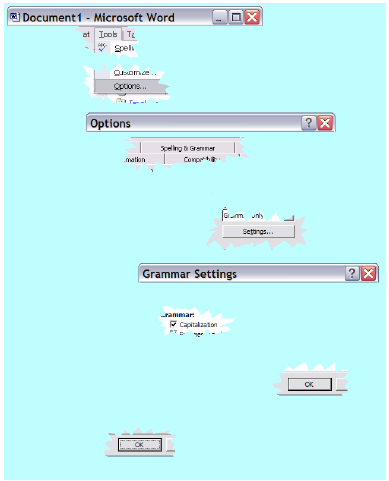
\includegraphics[width=0.7\textwidth]{graphstract}
	\caption[\emph{Graphstract} example]{An example of stepwise instructions in \emph{Graphstract} in the form of screenshot snippets, showing the steps required to toggle auto-capitalization in Microsoft Word. \emph{Image source:~\cite{huang:graphstract}}}
	\label{fig:graphstract}
\end{figure}

\noindent
Three iterations of user studies on a prototype is conducted by the authors, showing that \emph{Graphstract} performs better than conventional approaches overall, if not in all cases. They also conclude that adding text to the images is useful in many situations, despite their approach relying on graphical help only.

\subsection{Photo Tutorials}
\label{sec:photo_tutorials}
The authors of the paper \emph{Generating Photo Manipulation Tutorials by Demonstration}~\cite{grabler:photo_tutorials} argue the use of static visual tutorials (stepwise text-based tutorials accompanied by graphics) over video-tutorials for image processing software.

\noindent
In their work, the authors design a system for auto-generating static visual tutorials for a specific software product. These tutorials provide stepwise instructions with screenshots for completing a particular task, and additionally highlight the parts of the screenshots that are relevant to this task, as seen in Fig~\ref{fig:photo_tutorials}. This is combined with macros for automatic image labeling, to identify important regions of the particular image the user is working with.

\begin{figure}[htp]
	\centering
	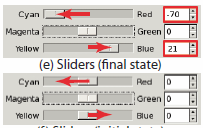
\includegraphics[width=0.5\textwidth]{photo_tutorials}
	\caption[\emph{Photo Tutorials} example]{An example of highlighting relevant \gls{ui} elements in a screenshot with \emph{Photo Tutorials}. \emph{Image source:~\cite{grabler:photo_tutorials}}}
	\label{fig:photo_tutorials}
\end{figure}

\noindent
Through a user study, the authors verify the effectiveness of their tutorials by observing that users perform significantly better and make less errors compared to tutorials based on text and video. However, some problem areas are identified: better tutorials can be created by providing feedback to users as they are performing the steps of the tutorial.

\subsection{Toolclips}
\label{sec:toolclips}
The authors of the paper \emph{ToolClips: An Investigation of Contextual
Video Assistance for Functionality Understanding}~\cite{grossman:toolclips} explore the \emph{learnability} of software products, more specifically relating to the concept of \emph{understanding} how to properly use functionality (see~\cite{grossman:software_learnability}). They identify problems with existing approaches based on both text and videos, where information is provided outside the context of the \gls{ui} in question. The authors also assess that regular tooltips, which provide the user with a short in-context description of what a \gls{ui} element does, do not provide a sufficient level of detail for complex tools.

\noindent
Attempting to provide the best of several worlds, the authors suggest their \emph{ToolClips} approach, enhancing regular tooltips with additional documentation and video content, in a more context-sensitive manner, as seen in Fig.~\ref{fig:toolclips}.

\begin{figure}[htp]
	\centering
	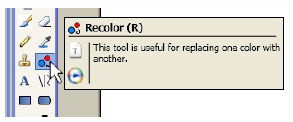
\includegraphics[width=0.7\textwidth]{toolclips}
	\caption[\emph{ToolClips} example]{An example of a \emph{ToolClip}, appearing as a regular tooltip, but with buttons allowing access to additional media. \emph{Image source:~\cite{grossman:toolclips}}}
	\label{fig:toolclips}
\end{figure}

\noindent
Through the results of two user studies, the authors show that the \emph{ToolClips} approach significantly improves users' understanding of how to use elements, and additionally has a positive impact on retention of this understanding, for applications that are \emph{highly graphical}.

\subsection{A Summary of Good Practices for Tutorials}
\label{sec:good_practices_tutorials}
The previous sections in this chapter, as well as Sect.~\ref{sec:tutorials}, describe various research efforts on the creation of good tutorials and introductions for computer-based procedures. Different aspects of the learning process are considered, and it is apparent that there are many ways to succeed. In this section, I attempt to summarize the various aspects that should be considered when making a tutorial for a computer-based procedure.

\paragraph{Interactivity and Active Learning} The most important aspect of a good tutorial is likely that it should be interactive. Active learning is one of Chickering and Gamson's \emph{seven principles of learning}~\cite{chickering:seven_principles}, in addition to being recommended for tutorial design by various other sources~\cite{bowerman:tutorial_design, aberson:tutorial_evaluation}. A common way of making a tutorial interactive is to provide exercises the user must complete.

\paragraph{Feedback} If a user is presented with tasks and exercises during the tutorial, it should also be possible to see the results of these exercises, and if applicable, check if the results are correct~\cite{chickering:seven_principles}. The feedback should also give the user some indication of the user's performance compared to the learning objectives~\cite{bowerman:tutorial_design}.

\paragraph{Motivation} It is important for users to know not only why they should learn the processes described in the tutorial (i.e. how these processes are useful to them), but also why they should complete more advanced tutorials on the subject that may optimize their work~\cite{grossman:software_learnability}. Users should also be informed of the scope of the tutorial, and what they are supposed to learn~\cite{bowerman:tutorial_design}.

\paragraph{Reasonable Teaching Order} If a tutorial teaches multiple concepts, a reasonable teaching order should be established, particularly if these concepts build on each other~\cite{bowerman:tutorial_design}. When deciding on a starting point, user' background must also be considered.

\paragraph{Context-sensitivity of Information} All new information presented in the tutorial should be provided at the point where it is actually needed, as opposed to being presented in an introduction part before the tutorial starts~\cite{andersen:tutorials_impact}.

\paragraph{Visual Mapping of UI Elements} If \gls{ui} elements are referenced in the textual part of a tutorial, it should be easy to map these references to the actual \gls{ui}. This can be done by adding (partial) screenshots of the \gls{ui}~\cite{huang:graphstract}, or highlighting the elements that are relevant for the current step~\cite{kelleher:stencils, bergman:docwizards, grabler:photo_tutorials}.

\paragraph{Multimedia Content} A tutorial that consists of text alone is rarely adequate, and can be improved by adding multimedia content such as images, sound, or video~\cite{grossman:software_learnability}. This kind of multimedia information content can also be present in the application itself, providing the user with more resources when help is needed~\cite{grossman:toolclips}. Animations can also be advantageous, but should be used only where natural, for example to describe events in time~\cite{morrison:animation}.

\paragraph{Help-on-demand} While the user generally shouldn't have to read through too much text before starting the interactive part of the tutorial, additional information resources should be available for when the user gets stuck, or for other reasons needs to know more about a specific topic~\cite{andersen:tutorials_impact, grossman:toolclips}.

\paragraph{Relevant Tasks} When a tutorial contains tasks and exercises, these should be as relevant as possible to the user, as opposed to fictional tasks created only for learning purposes~\cite{kelleher:stencils}.

\paragraph{High Expectations} Users should be presented with high expectations from the beginning, so that they are prepared to make an effort in understanding the concepts taught by the tutorial~\cite{chickering:seven_principles}.

\paragraph{Address Misconceptions} If common misconceptions exist within the topic that is being taught, the tutorial should do its best to address these misconceptions, preferably before they even have a chance to form~\cite{aberson:tutorial_evaluation}.

\paragraph{Multiple Perspectives} Generally, we want the user to actually think reflectively about the topic being taught, and not just passively absorb the facts. One way of doing this is by offering multiple perspectives of various concepts~\cite{aberson:tutorial_evaluation}.

\paragraph{Freedom} When introducing something like a game or a software product through a tutorial, we have to consider the amount of freedom users are given in the tutorial. There are issues in both allowing users complete freedom to explore, and restricting them to a single path~\cite{andersen:tutorials_impact, bonawitz:double_edged_pedagogy}. The optimal solution likely lies somewhere in between, by for example offering \emph{directed exploration}~\cite{esper:codespells}. 

\section{Learning With Games}
\label{sec:learning_with_games}
Most video games require the player to learn something in order to complete the game, whether it is difficult concepts like solving obscure puzzles, or simply the controls of the game. In some cases, games are even used to teach concepts for educational purposes, such as programming. In other cases, games even teach players valuable real-life skills without being deliberately designed to do so. The following sections briefly describe some of the efforts previously made in the field of educational games.

\subsection{Karel the Robot}
\label{sec:karel_the_robot}
Karel the Robot~\cite{pattis:karel_the_robot} is a game-like programming language and environment designed to teach basic programming concepts to beginners. It was developed by Richard E. Pattis in 1981, who used Karel to teach programming courses at Stanford University.

\noindent
The motivation behind Karel was to be able to teach students the basics programming without having to worry about the more complex and less important (to beginners) details. In Pattis' own words: \emph{``The careful omission of variables and data structures from Karel's language ... allows the immediate exploration of the rich domain of abstraction and control structures.''}~\cite{pattis:karel_the_robot}. This allows students to focus on learning how to solve problems through programming concepts.

\noindent
Karel was originally designed as a Pascal-like procedural programming language, but the concept gained wide popularity, and has been extended to Java~\cite{roberts:karel_the_robot_java},
Python,\footnote{\url{http://gvr.sourceforge.net/}}$^{,}$\footnote{\url{https://code.google.com/p/rur-ple/}} Karel++ (object-orientation)~\cite{bergin:karel_plus_plus}, REALbasic,\footnote{\url{http://www.ohloh.net/p/rbkarel}} and Scratch.\footnote{\url{http://scratched.media.mit.edu/resources/karel-robot-scratch}} Karel was inspired by the LOGO project,\footnote{\url{http://el.media.mit.edu/logo-foundation/index.html}} and has in turn inspired games like RoboMind\footnote{\url{http://www.robomind.net/en/index.html}} and C-Sheep~\cite{anderson:c-sheep}.

\noindent
The purpose of the game is to control a robot (Karel) by giving it a set of commands, and perform tasks. Initially, only a small set of commands are available, but as part of the learning process, users must learn how to extend these commands. The simplest task Karel is asked to perform is to pick up a beeper, seen as the diamond shape in Fig.~\ref{fig:karel_the_robot}.

\begin{figure}[htp]
	\centering
	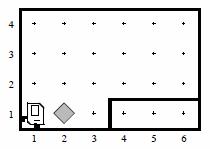
\includegraphics[scale=0.80]{karel_the_robot}
	\caption[Karel the Robot]{A simple \emph{Karel the Robot} level, where Karel (bottom left) must move to and pick up a single beeper (diamond shape). \emph{Image source:~\cite{roberts:karel_the_robot_java}}}
	\label{fig:karel_the_robot}
\end{figure}

\noindent
Karel the Robot has now been around for more than 30 years, and the teaching paradigm described has proved successful in introducing students to the art of programming.\footnote{See for example~\cite{krause:computer_science_air_force},~\cite{untch:karel_conventional_language},~\cite{becker:teaching_with_karel}} Students are allowed to explore advanced concepts in a safe environment with less relevant complexities removed, and in a way that makes them \emph{want} to learn. The concept has been adapted and refined in many ways over the years, but the core paradigm remains.

\subsection{Josef the Robot}
\label{sec:josef_the_robot}
Josef the Robot~\cite{tomek:josef_the_robot} is a game-like programming environment similar to Karel (Sect.~\ref{sec:karel_the_robot}). Unlike Karel, Josef more closely resembles ``real'' programming languages by being rich in structures and operations. Like Karel, Josef is also inspired by the LOGO project.

\noindent
The author of Josef, Ivan Tomek, provides ample motivation for creating a more novice-friendly environment for learning how to program. Firstly, potential learners should find the problems they can solve with programming to be interesting, which is likely not the case (for the average person) with problems like sorting a sequence of numbers. Furthermore, novice programmers should not have to worry about the more complex rules that are not directly related to problem-solving, such as syntax and data handling.

\subsection{Serious and Epistemic Games}
\label{sec:serious_games}
Games that are designed for a purpose that is not pure entertainment are often called \emph{Serious Games}, a term likely popularized by \emph{The Serious Games Initiative}\footnote{\url{http://www.seriousgames.org/}} in 2002~\cite{djaouti:serious_games_origins}. This genre encompasses many different types of games, but a prime example of a serious game is the \emph{flight simulator}, a realistic type of game that exists in various forms, and is extensively used to teach pilots how to fly aircraft.

\noindent
The idea behind serious games is to improve student motivation and engagement by providing immersive learning experiences, similar to how many professions are taught. I can read a lot about woodworking, but in order to become a good carpenter, I must practice. Seeing actual results of my knowledge and skills in woodworking is also likely to be more enjoyable than simply imagining how it might look. Games can provide a similar kind of (simulated) hands-on experience for topics that are difficult or inconvenient to practice immersively, especially more abstract topics like math or computer programming, and this has also proved to be a more efficient learning method in many cases. Children especially learn and are better motivated by the kind of problem-solving we find in games, as opposed to traditional textbook learning~\cite{freitas:serious_games_new_paradigm}.

\noindent
Several organizations working with serious games exist. Some examples are the \emph{Serious Games Institute},\footnote{\url{http://www.seriousgamesinstitute.co.uk/}} the \emph{Games Learning Society},\footnote{\url{http://www.gameslearningsociety.org/}} the \emph{Learning Games Network},\footnote{\url{http://learninggamesnetwork.org/}} and \emph{Serious Games Interactive}.\footnote{\url{http://www.seriousgames.net/}} These represent both commercial, societal, and academic interest in serious games.

\noindent
Researchers at the University of Wisconsin coined the term \emph{Epistemic Games} for the subset of serious games that aim to teach specific professions or skills~\cite{shaffer:epistemic_games}. They argue that games can help teach students to apply their knowledge, instead of simply remembering, in addition to facilitate for \emph{innovative} learning. With this as a basis, \emph{The Games and Professional Simulations Research Consortium}\footnote{\url{http://edgaps.org/gaps/}} has been formed in order to solve educational challenges through games and simulations.

\subsection{CodeSpells}
\label{sec:codespells}
\emph{CodeSpells} is a project from the University of California, San Diego, that aims to teach Java programming through a wizardry game~\cite{esper:codespells}. The CodeSpells team draws inspiration from the \emph{epistemic games} concept, and their games immerses novice programmers in a world that connects abstract code (Fig.~\ref{fig:codespells_spell}) with visual and ``physical'' effects in the environment (Fig.~\ref{fig:codespells_fire}).

\begin{figure}[htp]
	\centering
	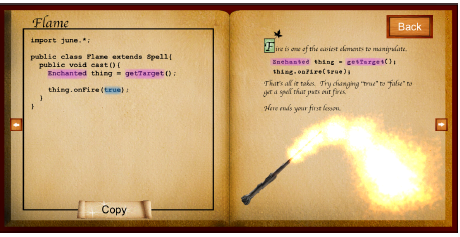
\includegraphics[scale=0.80]{codespells_spell}
	\caption[Java code for a CodeSpells spell]{An example of the CodeSpells spellbook, with Java code for the \emph{Flame} spell. The second page adds a short description, and a tip on how the spell can be modified. \emph{Image source:~\cite{esper:codespells}}}
	\label{fig:codespells_spell}
\end{figure}

\begin{figure}[htp]
	\centering
	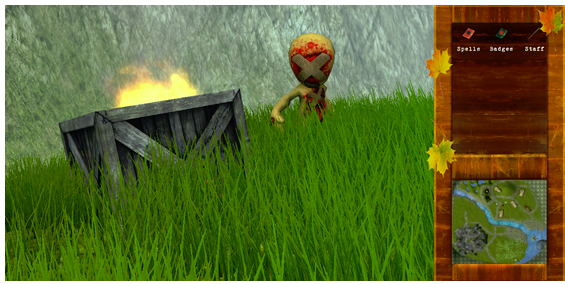
\includegraphics[scale=0.80]{codespells_fire}
	\caption[The CodeSpells game environment]{The game environment presented to the user in \emph{CodeSpells}. In this particular quest, the player must modify the \emph{Flame} spell (Fig.~\ref{fig:codespells_spell}) in order to extinguish the fire by setting \emph{thing.onFire(false)}. Image source: \emph{\url{https://sites.google.com/a/eng.ucsd.edu/codespells/home/level-1-quests}}}
	\label{fig:codespells_fire}
\end{figure}

\noindent
An important goal for the CodeSpells project is for students to gain a deep understanding of the programming language they use and problems they solve, and retain this understanding after completing the game. They would also like the students to be able to play the game without instructor assistance, and have focused extensively on designing quests that provide the appropriate scaffolding, as well as encourage exploration beyond the minimum required to move on~\cite{esper:design_quests_java_concepts}.

\noindent
In order to verify and improve the usefulness of their game for teaching programming, the CodeSpells team have conducted some user studies. Through these studies, they discovered that by immersing users in the game, the users developed a determination and a positive outlook on solving programming challenges~\cite{esper:codespells}. The team also discovered some principles that can be used to improve quest design~\cite{esper:design_quests_java_concepts}:

\begin{itemize}
	\item Provide examples that can be tested and used as a starting point, allowing users to see their effects.
	\item While the introduction should make it possible to perform complex actions with little effort, expectations for more effort should be provided from the beginning, letting users know that they have to build on and modify the examples.
	\item Provide directed exploration through quests, so the user can get a sense of complexity ordering and a choice of which challenge to overcome.
\end{itemize}

\noindent
These principles can likely also be used to improve design of other serious games.

\subsection{Non-Serious Games}
\label{sec:non-serious_games}
While the term \emph{Serious Games} covers the type of games that are designed for purposes other than entertainment, there are many examples of games designed for entertainment that ``accidentally'' teach their players valuable skills and knowledge.

\noindent
James P. Gee is a famous advocate for game-based learning. Through his analysis of various ``non-serious'' games, he identifies good principles of learning present in many of these games~\cite{gee:learning_machines}:

\begin{itemize}
	\item{\textbf{Empowered Learners:}} Players feel like active agents while playing, and not just passive recipients of information. Games are interactive, which leads to perceived ownership and engaged participation.
	\item{\textbf{Customization:}} Players are in many cases allowed to make choices about how to play, such as adjusting difficulty or playing style. People are different, and learn in different ways.
	\item{\textbf{Identity:}} Players often take on new identities within the game, in which they become heavily invested. This leads to a level of commitment that facilitates for deep learning.
	\item{\textbf{Manipulation and Distributed Knowledge:}} When players are able to control and manipulate a character or an object in the game environment, they feel expanded and empowered. Often, part of the knowledge required for manipulation is stored in the game itself (automated), so that the player can focus on the parts that are important for their task (and ``level of abstraction'').
	\item{\textbf{Well-ordered Problems:}} Players are exposed to problems in a well-ordered manner, so that they can form hypotheses that not only work in the moment, but prepare them for more difficult challenges later in the game.
	\item{\textbf{Pleasant Frustration:}} Players are exposed to problems that are neither too easy or too hard, but at the edge of the players' competence, and at their own pace.
	\item{\textbf{Cycles of Expertise:}} Players are allowed to repeat and practice skills until they become nearly automatic. Then, as the game progresses, they might have to adapt their skills to new conditions, and repeat the cycle.
	\item{\textbf{Context-sensitivity of Information:}} Players are often presented with the information they need \emph{when} they need it, instead of having to memorize it in advance.
	\item{\textbf{Fish Tanks:}} In many cases, games serve as simplified versions of real-world systems, and illustrate some important concepts while hiding complexities that might be too difficult to handle for novices. Sometimes, such fish tanks are also created within the game itself, in the form of tutorials. This allows players to exercise their skills without having to worry about \emph{all} the details.
	\item{\textbf{Sandboxes:}} Games also provide a safe environment for exercising skills, where the cost of failure generally is low compared to the real world.
	\item{\textbf{Skills as Strategies:}} Instead of practicing for the sole purpose of becoming good, players see the skills they learn as a strategy towards accomplishing goals within the game. This provides better motivation by allowing ``in-context'' practice.
	\item{\textbf{System Thinking:}} Many games consist of smaller elements, where players must understand how all the elements interact fit into the overall system of the game.
	\item{\textbf{Meaning as Action Image:}} Instead of just providing definitions and descriptions, games present concepts through visualizations and experiences, which is closer to how people actually think.
\end{itemize}

\noindent
These are clearly principles that should be considered also in serious and educational games, not only those made for entertainment. As Gee points out, \emph{``When we think of games, we think of fun. When we think of learning, we think of work''}. If done right, it is likely possible to merge the tedious process of learning with the fun of games with equal or better results.

\subsection{A Summary of Good Practices for Educational Games}
\label{sec:good_practices_games}
While educational games by default generally incorporate some good learning practices (interactivity and feedback), some ways of designing and implementing such a game are likely better than other. Based on the work described in the previous sections as well as Sect.~\ref{sec:game_based_learning}, this section summarizes some additional aspects that should be considered when designing an educational game.

\paragraph{Tutorials} Many games start by guiding the player through a tutorial in order to learn the basics of the game, which is similar to completing a tutorial in order to learn about a topic like programming language. Games, particularly complex ones, may benefit from having a tutorial introduction, in the form of increased player engagement~\cite{andersen:tutorials_impact}. Since educational games are often used to teach complex concepts, creating a tutorial is generally justified. The principles listed in Sect.~\ref{sec:good_practices_tutorials} also apply to tutorials for educational games, since these should be at least as good as tutorials for teaching a specific topic. Because of their immersive nature, video games likely makes a some of these principles easier to follow, such as providing good visual mapping of \gls{ui} elements and suitable multimedia content.

\paragraph{Immersion} By providing an \emph{immersive} experience, educational games can provide better motivation and encouragement for players to interact with and explore the concepts taught~\cite{esper:codespells}. Providing an immersive experience may include giving the player a sense of \emph{identity} in the game, enhancing commitment, or provide \emph{fish tanks} or \emph{sandboxes} where players can discover, explore, and experiment with concepts in safe and possibly simplified environments~\cite{gee:learning_machines}. Immersive game experiences also provide players with meaning for verbal concepts, through visualizations and experiences~\cite{gee:learning_machines}.

\paragraph{Exploration and Guidance} The discussion of exploration versus guidance becomes even more important for educational games than for tutorials. Good educational games often provide a safe environment where concepts can be explored and experimented with, even without any guidance. In many cases, too much guidance may even prevent exploration and discovery to some degree~\cite{bonawitz:double_edged_pedagogy}. Depending on the complexity of the concepts taught, having no guidance at all is also not a good solution. Some players will have more trouble than others understanding certain concepts, and subtleties are not always intuitively understood. The optimal solution is to evaluate the game's complexity, and provide some kind of middle ground (directed exploration,~\cite{esper:design_quests_java_concepts}) tailored not only to how difficult the concepts are, but the player's previous knowledge and ability to understand them. Users may even be allowed to choose their own difficulty level based on their own perceived experience level and skill.

\paragraph{Simplicity and Challenge} Irrespective of their background, any users within the target audience should be able to get started and see results early in the introduction~\cite{esper:design_quests_java_concepts}. However, the problems presented must eventually become difficult enough to allow players to gain deep understanding of the concepts taught, and expectations of this should be present from the beginning. Additionally, players can progressively be presented with an environment that is more and more like a real environment. This can help make the transition from practicing skills in a video game, to using these skills in real situations smoother~\cite{untch:karel_conventional_language}.

\cleardoublepage
\chapter{A Tutorial for UML Activities in Reactive Blocks}
\label{ch:reactive_blocks_tutorial}
As the first part of my own work, I set out to make a set of tutorial exercises for learning to create \gls{uml} Activity diagrams in Reactive Blocks. This chapter begins by describing the motivation behind and goals for this set of exercises. A tutorial design is then proposed, followed by a description of and results from a user study.

\section{Motivation}
\label{sec:tutorial_motivation}
Before setting out to create a tutorial for \gls{uml} Activities in Reactive Blocks, it is important to determine if there is real motivation for this. If good tutorials already exist, another is likely redundant. While it is certain that \emph{some} tutorials exist, we also need to check if these adhere to the principles of good tutorials discussed in Sect.~\ref{sec:good_practices_tutorials}. If there is motivation for creating a new and better tutorial, we should establish some goals and guidelines in advance.

\subsection{Existing Tutorials}
\label{sec:existing_tutorials}
The major part of the motivation for creating a set of tutorial exercises comes from looking at the tutorials that already exist for \gls{uml} Activities and Reactive Blocks. While these tutorials generally present the information required to get started, it is not necessarily presented in an optimal way to newcomers.

\subsubsection{Tutorials for UML Activities}
The official \gls{uml} website\footnote{\href{http://www.uml.org/\#Links-Tutorials}{Unified Modeling Language Resource Page (link)}} links to four sources of tutorials for learning about \gls{uml}:

\begin{itemize}
	\item{\textbf{No Magic \emph{MagicDraw}:}} Not really a tutorial, but a commercial software product for software modeling. A quick inspection of the trial version does not reveal any tutorial functionality other than some tips for using the software.
	\item{\textbf{\gls{omg}'s List of Training:}} Also not a tutorial, but a list of companies that offer UML training. Mostly as n-day sessions on-site.
	\item{\textbf{Mario Jeckle - UML Tutorials:}} A German website with a lot of links to other sources of information, many of which do not even work.
	\item{\textbf{Sparx Systems:}} The only link that actually leads to something resembling a tutorial. However, information is presented in a more documentation-like way, ignoring most practices for good tutorials.
\end{itemize}

\noindent
A quick Google-search lists some additional tutorial sources, but most follow a documentation-like approach similar to the one from Sparx Systems listed above. In short, there is a real lack of interactive \gls{uml} tutorials, where the user gets to learn a few concepts at a time, and to use and understand these concepts in the context of examples and exercises.

\subsubsection{The Reactive Blocks Tutorials}
Reactive Blocks has a set of tutorial exercises available to new users of the software.\footnote{\href{http://reference.bitreactive.com/tutorials/}{Reactive Blocks Tutorials (link, requires registration)}} These tutorials are created in an exercise-like manner, where the user is presented with some new information, and must use this in examples. However, the tutorials are mostly focused around the capabilities of the software and how to use it, rather than teaching good modeling. Previous familiarity with \gls{uml} Activities seems to be assumed.

\noindent
If one is to learn about \gls{uml} Activities through Reactive Blocks, an additional set of tutorials must likely be made, with primary focus on the modeling aspect. In addition, like with the existing tutorials, it is likely that some information about using the software must be included.

\subsection{The Target Audience}
\label{sec:target_audience}
Making a tutorial that works well for \emph{anyone} is difficult, maybe even impossible. The interest for a tutorial like this is also likely to be limited to a relatively small number of people, more specifically those who want to learn how to use \gls{uml} Activities, or even Reactive Blocks, to improve or simplify their software development process. This provides a rough frame for our target audience.

\noindent
It is important to note that while people in the target audience likely have similar goals, their background and previous knowledge may vary. Users may be complete beginners in the field of programming and software development, experts simply seeking to add another tool to their process, or anything in between. The whole range of backgrounds and previous knowledge should be taken into consideration when designing and implementing the tutorial.

\subsection{Goals}
\label{sec:tutorial_goals}
This section outlines the goals I set before creating the tutorial.

\paragraph{Focus on UML Activities} If the user wants to learn how to work with Reactive Blocks, learning about \gls{uml} Activities is a start, but far from sufficient. The scope of this project is however learning modeling languages, so the tutorial should focus on the modeling aspect, and deal with topics specific to Reactive Blocks only where absolutely needed. This includes dealing with Java code; all operations required in a model should be predefined.

\paragraph{Avoid Irrelevant Complexities} Reactive Blocks is a full-fledged modeling and code generation tool, with capabilities that go way beyond simply modeling \gls{uml} activities. This gives the tutorial some advantages, such as actually creating runnable code from the models created, which provides the user with relevant feedback. However, it also introduces complexities that are not as relevant when learning about \gls{uml} Activities. Ideally, Reactive Blocks should have a separate tutorial mode that handles these additional complexities, and lets the user focus on the modeling.

\paragraph{Difficulty and Challenges} The exercises presented to the user should be easy enough to allow most users to complete them without much difficulty and frustration, while still communicating the lesson properly. In addition, there should be challenges, perhaps as supplementary exercises, that force the users to really think about how an element can be used, and lets them take on a different perspective for solving the problem.

\paragraph{Everything in One Place} With online tutorials, users often have to change between the application window, the tutorial (often in a web browser), and any other necessary resources. This increases the short-term memory workload, since users have to remember a lot of information between the windows. One of the golden rules of \gls{ui} design is to reduce the short-term memory load~\cite{shneiderman:user_interface}, so for the tutorial, I would like to provide all the information and parts of the tutorial within Reactive Blocks, letting users find the resources they need while still being able to see the current problem. This should also help create some sense of immersion, though a standard tutorial will most likely not be nearly as immersive as a video game in any case.

\paragraph{Follow the Principles of Good Tutorials} Section~\ref{sec:good_practices_tutorials} summarizes various practices for making good tutorials. I would like to follow these as much as possible, while at the same time acknowledging that I likely will not be able to cover all. The ones I consider most relevant for this tutorial are:

\begin{itemize}
	\item{\textbf{Interactivity and Active Learning:}} The tutorial should first and foremost be interactive. For each new piece of information introduced, users should be presented with exercises they have to solve.
	\item{\textbf{Feedback:}} Users should be given feedback on their exercises. Fortunately, using Reactive Blocks is a big help here, since the tool makes it possible to actually run the models created. In this way, users can see if their programs behave as expected.
	\item{\textbf{Reasonable Teaching Order:}} Instead of learning everything about \gls{uml} Activities in one step, I would like to introduce one new element at a time, starting with the most basic elements like edges and operations. Then I will add a few more elements at a time, while allowing the users to experiment a little with the new elements for each step.
	\item{\textbf{Context-sensitivity of Information:}} Instead of providing a complete documentation for \gls{uml} Activities at the beginning and then start off with exercises, I would like to document each new element in the exercise where they are introduced, i.e. in-context.
	\item{\textbf{Help-on-demand:}} It is not a good idea to force readers to read through every detail about something before they start getting familiar with it, but I would like information about every detail to be available on-demand should the user need it.
	\item{\textbf{Visual Mapping of \gls{ui} Elements:}} Eclipse is a tool used in many aspects of software development, and most parts of it will not be relevant to this tutorial. Whenever parts of the Eclipse and Reactive Blocks interface are referenced, the tutorial should make them easy to find.
	\item{\textbf{Multiple Perspectives:}} \gls{uml} Activities and Reactive Blocks can be used to model many different kinds of systems, and it is important to understand their capabilities. The tutorial should provide exercises that use the various elements in different contexts and with different purposes, when applicable.
	\item{\textbf{Freedom:}} Because the tutorial is made with Reactive Blocks, it is likely a good idea to limit the users' freedom when working with the tutorial. It is easy to get confused by the many capabilities of Eclipse and Reactive Blocks, and clicking the wrong thing can easily lead to unexpected errors. Having a separate tutorial mode is one possible way of doing this. At the same time, we do not want to restrict the users to one specific way of thinking when solving the tutorial exercises. Ideally, it should be possible to solve these exercises in more than one way, and the users should be made aware of this.
\end{itemize}

\noindent
These goals provide a basis for the design of the tutorial, and will hopefully lead to a tutorial that introduces \gls{uml} Activities to novices in a better way than the existing tutorials described in Sect.~\ref{sec:existing_tutorials}.

\section{Tutorial Design}
\label{sec:tutorial_design}
The tutorial design consists of three parts:

\begin{itemize}
	\item An enhanced Reactive Blocks user interface, i.e. a \emph{tutorial mode}.
	\item A teaching order for the various elements and concepts, with an introduction for each new element and concept.
	\item An exercise for each step in the tutorial, implemented in Reactive Blocks. Some steps additionally have a challenge exercise.
\end{itemize}

\subsection{Proposal for a Reactive Blocks Tutorial Mode}
\label{sec:reactive_blocks_tutorial_mode}
The first part of the tutorial design is a proposal for a \emph{tutorial mode} in Reactive Blocks. Figure~\ref{fig:tutorial_mode} displays a visual mock-up of the proposed \gls{ui} design for the tutorial mode. In the middle, we see the familiar Reactive Blocks modeling canvas (10), with some elements in place for demonstrative purposes. Surrounding the modeling canvas, we see various new elements that will be explained below.

\begin{figure}[htp]
	\centering
	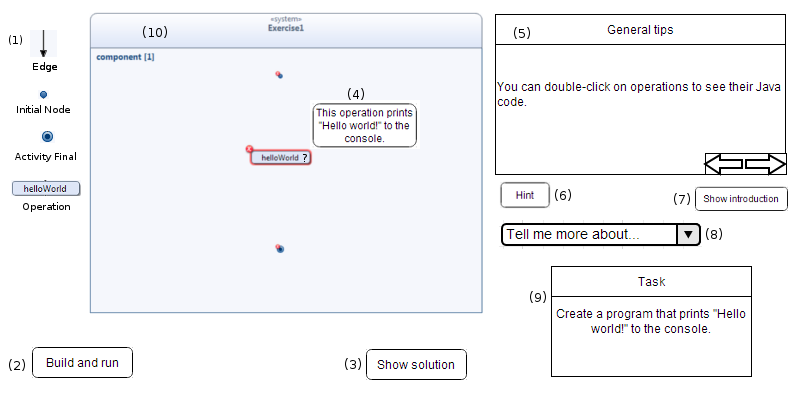
\includegraphics[width=\textwidth]{tutorial_mode}
	\caption[Reactive Blocks tutorial mode design]{A visual mock-up of the UI presented to users when running Reactive Blocks in the suggested tutorial mode. The regular modeling canvas is shown in the middle (10), surrounded by utility buttons and three information windows.}
	\label{fig:tutorial_mode}
\end{figure}

\paragraph{Element Buttons (1):} Instead of the current right-click menu selection scheme for adding elements to the canvas, buttons for each type of element is placed on the side, allowing more \emph{direct manipulation}. The modeling canvas allows direct manipulation of elements already present, but allowing user to add new elements in the same way is likely to make an introduction to the software smoother and quicker for novices~\cite{shneiderman:user_interface}.

\noindent
We should also note that only a few of the possible modeling elements are present. This is meant as a way of hiding extra complexity, by only displaying the elements that have been introduced so far in the tutorial. Other elements are still available via the right-click menu.

\paragraph{\emph{Build and Run} Button (2):} In order to see the results of running a program, users have to first \emph{build} their model (generate executable code) and then run it. Learning how to do this involves several steps, such as navigating drop-down menus and choosing Java platform (see the ``Building and running the exercises'' part of Appx.~\ref{appx:tutorial}), While highly relevant when learning to work with Reactive Blocks, this process adds complexity that is less relevant for learning to work with \gls{uml} Activities. The purpose of the button is to remove the complexities by automatically performing the needed operations to run and build the model, with some default options that work with the tutorial. Like the element buttons, this button also allows more \emph{direct manipulation}.

\paragraph{\emph{Show Solution} Button (3):} In some cases, users may be unable to progress in a tutorial because they get stuck at certain steps. In this case, it is natural to ask for help from an instructor, but we would like users to be able to complete the tutorial without outside help. One way of doing this is to allow the users to see the solution to an exercise (in a pop-up window) when they are unable to complete it. Ideally, this button should only become visible after a certain time has passed, so as not to tempt the user into checking the solution before a serious attempt at finding it has been made.

\noindent
An additional advantage is that when multiple solutions are possible, the user may discover a different approach than the one proposed, offering multiple perspectives to the same concept. To this end, a solution can be provided to the user even in cases of success, allowing comparison of solutions and additional reflection.

\paragraph{Information about operations (4):} One of the goals for the tutorial was to avoid users having to deal with Java code, as this adds complexity that is less relevant to learning about \gls{uml} Activities. The users still need to know what the predefined operations they are using in their models actually do, and the name is not always enough of a description. The tutorial mode adds a clickable ``?'' on the operation icon, which opens a sticky note providing a short description of what the operation does. The sticky note is then removed when the user clicks somewhere else.

\paragraph{\emph{General Tips} Window (5):} This window provides the users with some general tips on how to work with Reactive Blocks and \gls{uml} Activities. These should not be necessary to complete the tutorial, but may provide more interested or advanced users with some additional information about what goes on behind the curtains. Their purpose is also to ease the transition towards working with Reactive Blocks without the training wheels provided by the tutorial, for users to whom this is relevant.

\paragraph{\emph{Hint} Button (6):} Like the \emph{Show Solution}
button, the purpose of the \emph{Hint} button is to provide users that are unable to complete the tutorial on their own with some help. Unlike the solution however, this button is always visible. The hints provided should not give away the solution, but rather offer some insight about the task, concepts, or elements presented, that may not be obvious to all users.

\paragraph{\emph{Show Introduction} Button (7):} An important part of the tutorial is the introduction, which is provided at each step. The introduction gives the user some basic information about the new concepts and elements introduced at the current step, allowing the user to understand and use the elements and concepts to complete the task. Since activity steps in Reactive Blocks describe events in time, it is natural to use animation to communicate this information~\cite{morrison:animation}, perhaps supplemented by audio or textual descriptions. This animation is displayed when the user first enters the step, and the button allows the user to review the animation when this is needed.

\paragraph{\emph{Tell me more about...} drop-down menu (8):} This menu serves as the \emph{help-on-demand} part of the tutorial. In the menu, the user can select various concepts and elements to see more extensive and detailed information about them, either in an embedded pop-up window or through external resources, such as online documentation.

\paragraph{\emph{Task} Window (9):} This window simply shows the task the user needs to complete for the current step.

\noindent
Unfortunately, Reactive Blocks is a closed source product, meaning I was not able to implement and test this tutorial mode design. It is however still highly relevant to the thesis, as it was supposed to cover several of the good practices for tutorials, and serves as a basis for the \gls{ui} presented in the game in Ch.~\ref{ch:tutorial_game}.

\noindent
Since I was not able to implement this design in Reactive Blocks, I had to give up some of the goals I set for the tutorial. I was, for example, not able to provide \emph{everything in one place}. The tasks and exercises were still implemented in Reactive Blocks, but the introductions and information about concepts and elements had to be provided in a separate document (see Appx.~\ref{appx:tutorial}) and as text and images only, not animations. In addition, it was difficult to provide \emph{solutions} to the exercises, and instead of abstracting away the process of \emph{building and running}, a description of how to do it manually was added. In the end, there was more focus on learning processes specific to Reactive Blocks than originally intended. Help-on-demand was only offered by a reference to the official online documentation.

\subsection{Teaching Order}
\label{sec:teaching_order}
Teaching users to model systems with \gls{uml} Activities and Reactive Blocks includes teaching how to use the various modeling elements as well as introducing more abstract concepts, like activity steps, looping and modularity.

\noindent
Finding a good teaching order was challenging, but after a lot of consideration and testing of exercise ideas, I settled on the order displayed in Tab.~\ref{tab:teaching_order}. Each step teaches a new concept that is central to \gls{uml} Activity Modeling, and introduces some elements that can be used to implement this concept.

\begin{table}[htp]
	\centering
	\begin{tabulary}{\textwidth}{| C | C | C |}
		\hline
		\textbf{Step number} & \textbf{Concepts} & \textbf{Elements} \\
		\hline
		1 & Control Tokens, Activity Steps & Initial Node, Operation, Activity Final, Edge \\
		\hline
		2 & Stable Position & Timers \\
		\hline
		3 & Alternate Branches & Decision, Object Flow \\
		\hline
		4 & Looping & Merge, Flow Break \\
		\hline
		5 & Parallelism and Concurrency & Fork, Event Reception \\
		\hline
		6 & Synchronization & Join \\
		\hline
		7 & Modularization & Local Block \\
		\hline
	\end{tabulary}
	\caption[UML Activities Tutorial Teaching Order]{The teaching order for the UML Activities Tutorial. Each step teaches a concept, and introduces one or more elements that can be used to implement the concept.}
	\label{tab:teaching_order}
\end{table}

\noindent
The reasons for the choice of ordering are explained below:

\begin{itemize}
	\item{\textbf{Step 1:}} This step introduces the core concepts and elements that are required for an application that does something the user can see the result of.
	\item{\textbf{Step 2:}} Timers were introduced in the second step, because they provide a simple and intuitive way of dividing a program into more than one activity step. They also need to be introduced before flow breaks.
	\item{\textbf{Step 3:}} This step introduces alternate branches and decisions. Branches must be introduced before loops, to provide a way of breaking the loop. Decisions also require the users to know about object flow, but this is also the first instance where this type of flow is needed.
	\item{\textbf{Step 4:}} This step introduces loops with merge nodes. Merge nodes are also very useful when working with concurrency. Loops must also be split into more than one step, which can be done elegantly and without adding delay by using the flow break.
	\item{\textbf{Step 5:}} Users should now be comfortable enough with basic concepts to start working with concurrency. Concurrent branches are also required before join nodes become useful.
	\item{\textbf{Step 6:}} The final core element to be introduced is the join node.
	\item{\textbf{Step 7:}} Modularization and local blocks are without doubt the most advanced concepts taught by this tutorial, because of how they are implemented in Reactive Blocks. Using a local block requires the user to learn an additional concept, \glspl{esm}, and if the user wants to make a new local block, input and output pins must be considered.
\end{itemize}

\noindent
For each new concept and element, a short textual introduction is provided. I attempted to make these descriptions as short as possible, while making sure they still covered the concepts adequately. \emph{Adequately} was entirely based on my own judgment, but the user test conducted in Sect.~\ref{sec:tutorial_testing} offers some insight into whether this was true.

\noindent
The complete tutorial document, with introduction text for each concept and element, is included in Appx.~\ref{appx:tutorial}.

\subsection{Tutorial Exercises}
\label{sec:tutorial_exercises}
For each of the seven steps described in Sect.~\ref{sec:teaching_order}, I designed and implemented an exercise in Reactive Blocks. The exercises were designed as unfinished blocks with predefined operations, which the user had to complete and then run to see if the result was correct. Some steps additionally had extra challenge exercises, which were optional but encouraged. This section describes each exercise and its purpose. The exercise project is also available online for download.\footnote{\href{https://github.com/Desarc/reactive-blocks-tutorials/tree/master/no.ntnu.item.tutorials}{Tutorial project on GitHub (link)}}

\subsubsection{Exercise 1 - Hello World!}
Everyone who has learned programming in any way has likely created a ``Hello World!'' program at some point. It is one of the simplest programs one can make, also in Reactive Blocks, and used as the first step of programming introductions almost universally. To students, this is likely to be a familiar example.

\paragraph{Task:} Create a ``Hello World!'' program.

\paragraph{Purpose:} Teach users about \emph{activity steps}, \emph{tokens}, \emph{edges}, and \emph{operations} with a very simple example. Users also have to use an \emph{Initial Node} to start the application. Use of the \emph{Activity Final} is optional, but users will hopefully discover that they have to terminate the program manually if this element is not included. Note that this exercise only demonstrates a single activity step, and likely does not offer sufficient understanding of this concept for later use.

\paragraph{Challenge exercise:} The challenge exercise asks users to create a program that prints one message, then a second message, then the first message again. The purpose is for users to (hopefully) discover that operations can be used more than once in the same \gls{uml} Activity diagram.

\subsubsection{Exercise 2 - Delays}
A very important aspect of \gls{uml} Activities is that activity steps are essentially atomic, meaning that logically there is zero delay between operations in the same step. Operations are also not allowed to wait or block, and while in reality each activity step takes some time to complete, they logically happen instantly. Delays are then used to provide waiting capabilities without blocking the application, allowing other steps to run in the meantime.

\paragraph{Task:} Create a program that displays a light, sets its color to red, then changes it from red to green after 5 seconds. Make sure you have time to see that the light has changed before the program terminates.

\paragraph{Purpose:} Teach users about \emph{timers}, \emph{stable positions} and multiple activity steps. This exercise only illustrates how timers can be used to implement delays, and not how they allow other parts of the program to run in the meantime.

\paragraph{Challenge exercise:} The challenge exercise asks users to create a more advanced traffic light, with several more steps and transitions. While strictly speaking equally complex and with no new perspective added, it gives the users more practice in working with timers. Users may also notice that the larger model requires a little more mental effort to set up and possibly debug.

\subsubsection{Exercise 3 - Choices}
Branching is an important concept in computer programming. Depending on specific data or events, one may want the program to behave differently. Reactive Blocks and \gls{uml} Activities also implements this concept, by allowing an activity step to take different paths, depending on some data that is carried by the active token.

\paragraph{Task:} Create a program that generates a random number between 0 and 200, and prints ``Small!'' if the number is smaller than 100, and ``Big!'' if the number is greater than 100.

\paragraph{Purpose:} Teach users about \emph{alternate branches}, \emph{decisions}, and \emph{object flow}. Users must learn how to pass data between elements in the diagram, and to set guards on the edges from a decision to decide which path the program should take.

\paragraph{Challenge exercise:} The challenge exercise asks users to find a given number by implementing a binary search tree. It requires some additional information about how to work with decisions, encouraging users to become familiar with their documentation.

\subsubsection{Exercise 4 - Looping}
Another important concept in computer programming is loops; repeating the same procedure many times. This concept can also be implemented in \gls{uml} Activities and Reactive Blocks, with the help of merge nodes.

\paragraph{Task:} Create a program that generates a random number between 0 and 200 until that number is greater than 100 (big).

\paragraph{Purpose:} Teach users about \emph{loops}, \emph{merge nodes}, and \emph{flow breaks}, which are timers with zero delay. An important point in this exercise is to learn that a token may only pass through an element \textbf{once} in each activity step, meaning loops must be split into separate steps for each iteration, for example by using a flow break.

\paragraph{Challenge exercise:} This step has no challenge exercise.

\subsubsection{Exercise 5 - User input and parallelism}
One of the big advantages of creating software with Reactive Blocks is that it is fairly easy to implement parallelism and concurrency. This is a central concept in \gls{uml} Activities, and visualized by forking a flow. Concurrency is particularly useful for receiving user input, where one part of the application may wait for input, while another part performs a different task.

\paragraph{Task:} Create a program that changes the color of a light every time you press one button, and exits when you press another. It should be possible to change the light an arbitrary number of times before exiting (even zero).

\paragraph{Purpose:} Teach users about \emph{parallel branches}, \emph{forks}, and \emph{events}. This exercise should hopefully improve users' understanding of activity steps and waiting, as introduced with timers in exercise 2, and additionally adds indefinite waiting with events.

\paragraph{Challenge exercise:} The challenge exercise for this step is to implement a simple game, where the user must navigate through a set of doors (full description available in Appx.~\ref{appx:tutorial}). The purpose of this challenge is to teach users to model ``larger'' systems, and combine most of the concepts learned so far. It is also meant to show users the power of being able to receive user input, and that it is possible to create programs that do not seem completely artificial, but actually do something \emph{useful}.

\subsubsection{Exercise 6 - Synchronization}
In many cases, we want to perform a task only when several concurrent tasks have been completed. In order to do this, we need some functionality that waits for all this tasks to complete before continuing. In Reactive Blocks, this is implemented with a \emph{join} node.

\paragraph{Task:} Create a program that prints a message and then terminates when three buttons have been clicked (in any order).

\paragraph{Purpose:} Teach users about \emph{synchronization of flows} and the \emph{join} node.

\paragraph{Challenge exercise:} This step has no challenge exercise.

\subsubsection{Exercise 7 - Modularization}
One of the most important concepts in \gls{uml} Activity modeling is modularization. When dealing with large and complex programs, we generally want to separate parts of the functionality into smaller modules, making the application as a whole more orderly, and allowing reuse. However, in the context of Reactive Blocks this introduces some additional complexities like \glspl{esm}, which may arguably be the most difficult concept to grasp for Reactive Blocks novices.

\paragraph{Task:} Use the \emph{Counter} block to make the \emph{CoinFlipper} block ``flip a coin'' 10 times, and then return the result.

\paragraph{Purpose:} Teach users about \emph{modularization} and \emph{local blocks}. This exercise is a huge step up from the previous exercises, since it introduces users to many subtleties in Reactive Blocks related to concepts like activity steps and \glspl{esm}.

\paragraph{Challenge exercise:} Since this tutorial was tested in the context of the TTM4115 course at \gls{ntnu}, students were directed to the first lab exercise of this course as the challenging part of this step. In this lab exercise, students must create their own local blocks with \glspl{esm}, and connect them to form a complete application.

\section{User Testing and Feedback}
\label{sec:tutorial_testing}
In order to verify the usefulness of this tutorial, I attempted to conduct a user test. It is not easy to find a sufficient number willing test subjects for a test like this, but being a student assistant in the TTM4115 course at \gls{ntnu}, where the students learn about \gls{uml} modeling and additionally need to use Reactive Blocks for their semester assignment, I had a unique chance to expose my tutorial to users that actually needed it.

\subsection{Testing Method}
\label{sec:tutorial_testing_method}
The testing method used was rather straightforward. I arranged a two hour session where the subjects could work the tutorial on their own, but I would be available for help if needed. Each test subject also received a feedback form they would anonymously fill out in the end, and hand back to me.

\noindent
I convinced the TTM4115 lecturers to let me use one of the weekly exercise sessions for the testing session, since the students needed to learn about Reactive Blocks for their assignments anyway. The students knew in advance that the particular session would be used for the tutorial, which actually led to more students showing up than usual. Initially I took this as a good sign, but it turned out many of them did not even know about the weekly exercise sessions before I showed up during a lecture and asked them to participate in my test. In addition to the testing session, the tutorial was made available online, for those who wanted to do it, but were unable to attend the session.

\noindent
Ideally, I should have conducted a standard A/B split test, where some users would complete my tutorial while others did the standard tutorials. This did not happen for several reasons, the primary reason being an overall low number of test subjects. Additionally, it would have been difficult for me to measure and compare results, because most of the test subjects were there in their own interest, and did not want to spend a lot of time on tests and surveys after having completed the tutorials. Students did have a choice in whether they wanted to do my tutorial or the standard tutorials, but because of endorsement from the course lecturers (mine ended up being the one featured on the course website), they all chose to do mine.

\noindent
During and after the testing session, I was able to gather data in three different ways:

\paragraph{Feedback forms} All the students who attended the testing session were handed a feedback form. Around 20 students attended the session, but only 11 handed in the form at the end. In addition, 2 students answered the online form. The complete feedback form is available in Appx.~\ref{appx:feedback_form}.

\noindent
The feedback form consists of 7 questions. The expected number of participants for the testing session was low, so the questions were not intended to provide data for quantitative analysis, but rather attempt to identify problematic areas in the tutorial, and if anything could be improved. Since the test subjects were present in their own interest, the form was kept brief in order to not scare them away from filling it in (a too long questionnaire may require more extra effort than the participants are willing to give).

\noindent
The first question asked whether the user found the introductions useful in solving the exercises. Positive answers were expected, but only negative answers would really have been interesting, since they could indicate that the introductions are in some way flawed, such as being redundant or lacking in information.

\noindent
The second question was intended to give some indication on how the subjects thought about learning concepts like these from a game, for future reference. If people think they will enjoy learning these concepts from a game, there is a stronger incentive to explore this way of learning.

\noindent
The third question asked whether the subjects by their own judgment felt that they understood the concepts presented in each exercise, rated by a degree of understanding for each exercise. Like with the first question, the interesting results would have been negative ones.

\noindent
The fourth question asked whether the subject completed the challenge exercises, which were optional. This was meant to measure the subjects' motivation and willingness for gaining a deeper understanding of the concepts presented.

\noindent
The fifth question asked the subjects to give an indication of the challenge exercises' difficulty. This question was slightly flawed, as it should have asked for separate feedback for each exercise. However, if most of the test subjects were to answer that the challenge exercises were, for example, too easy, this would give me something to consider for improvement.

\noindent
The sixth question asked why, if not, the subject did not complete the challenge exercises. If motivation and willingness to gain a deeper understanding was lacking, it would be useful to know why, in order to attempt at providing better and clearer incentive.

\noindent
The seventh and final questions simply asked for additional comments, so that subjects could add their own thoughts.

\paragraph{Observations during the session} Since I was present for help during the whole session, I was able to make various observations about what people seemed to struggle with, and which parts needed refinement.

\paragraph{Observations in the following weeks} As a student assistant in the course, I was present during all the following exercise sessions, where the students had to use Reactive Blocks to complete assignments. This allowed me to make some additional observations about what they had learned from the tutorial, but I did not know which of the students had actually completed the tutorial, so this was by all counts less reliable data. It did however give me some indication about what they \emph{needed} to learn from a tutorial.

\subsection{Test Results}
\label{sec:tutorial_test_results}
With the total number of test participants being low, a quantitative analysis of the tutorial's quality was out of the question. Instead, I use the results to look for areas with potential for improvement, or indications of what works well.

\subsubsection{Test Subject Profile}
All of the participants in the user test were students of the TTM4115 course at \gls{ntnu}.\footnote{\href{http://www.item.ntnu.no/academics/courses/ttm4115/start}{TTM4115 course website (link)}} Some of the participants were 3rd year students of the 5-year MSc in Communication Technology at \gls{ntnu}, while others were students of the 2-year MSc in Telematics. All were assumed to have some knowledge of computer programming or software design. Prior to the user test, the students had a 2-hour introduction lecture for \gls{uml} Activities in Reactive Blocks.

\subsubsection{Problems During the User Test Session}
Not everything went smoothly during the testing session, which caused some delays and some additional trouble for the participants. First of all, very few of the participants came prepared, and had to go through the process of installing Eclipse and Reactive Blocks before starting the tutorial. Some had trouble with this part, and needed help from me or my co-instructor. Additionally, a license is required in order to use Reactive Blocks, and not all participants had received one. Fortunately they were able to get one during the session, but at the cost of extra delay. Finally, there were some errors in the Reactive Blocks tutorial project I had not discovered, which had to be fixed on the fly and caused some additional delay.

\noindent
The testing session was only 2 hours, and as a result of the various delays, many of the participants were not able to complete the whole tutorial. This is likely the reason why many of the participants chose to not fill out the feedback form, and even from the few who did, there were several who did not complete the whole tutorial.

\subsubsection{Data from the Feedback Form}
I received a total of 13 filled out feedback forms during and after the testing session. This section summarizes the answers, and attempts to highlight the information we can infer from these results.

\paragraph{Question 1:} Figure~\ref{fig:feedback_form_q12} displays the results from question 1: \emph{``Did you find the provided information about elements and concepts useful?''}. All participants answered that they found the provided information about elements and concepts to be useful. This tells us that at least there is nothing that is apparently wrong with the introductions to the exercises, however it does not necessarily mean they are very good.

\paragraph{Question 2:} Figure~\ref{fig:feedback_form_q12} also displays the results from question 2: \emph{``Do you think you would find the exercises more interesting if they were designed as a game, where you had to create a program to complete each level?''}. Here the answers varied a little more, with 2 participants answering that they would not be interested in learning these concepts from a game, while 5 answered that it would depend on the type of game. The remaining 6 gave positive answers. In hindsight, it would have been interesting to know which types of games the 5 participants were interested in, but this is also the kind of question one might not know the answer to without seeing some examples. Overall, the results indicate that a well-designed game may improve motivation for at least some of the students. For the remaining, it is hard to say whether the game approach will reduce motivation or simply leave it unchanged.

\begin{figure}[htp]
	\subfloat{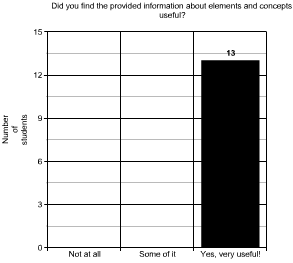
\includegraphics[width=.49\textwidth]{feedback_form_q1}}
	\subfloat{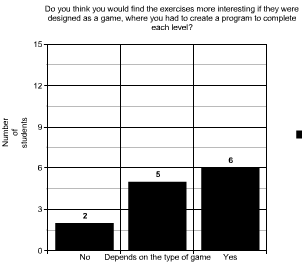
\includegraphics[width=.49\textwidth]{feedback_form_q2}}
	\caption[Results from feedback form questions 1 and 2]{Results from questions 1 (left) and 2 (right) of the feedback form (Appx.~\ref{appx:feedback_form}). The total number of students was 13.}
	\label{fig:feedback_form_q12}
\end{figure}

\paragraph{Question 3:} Figure~\ref{fig:feedback_form_q3} displays the results from question 3: \emph{``Did you feel that you understood the concepts presented in the exercise?''}. The results are displayed as a separate graph per exercise, where the participants had to rate their own understanding. The most important point to notice from these results is that more than half of the participants did not have time to complete exercise 5 through 7, and 3 of these also did not complete exercise 4. It is possible that these are students in the ``lower end of the bell curve'', who have more difficulty and take more time in grasping the concepts presented in the exercise. Looking at the results for exercise 1 and 2, all or nearly all of the participants felt that they completely understood the concepts presented. As we move on to exercise 3, some of the participants are beginning to reduce their perceived level of understanding to ``pretty good''. From the participants who completed exercise 4 through 6, all measured their own understanding to be complete, but in exercise 7 the results are slightly worse. It appears that the most challenging exercises are 3 and 7, and these may have to be revised and improved.

\begin{figure}[htp]
	\centering
	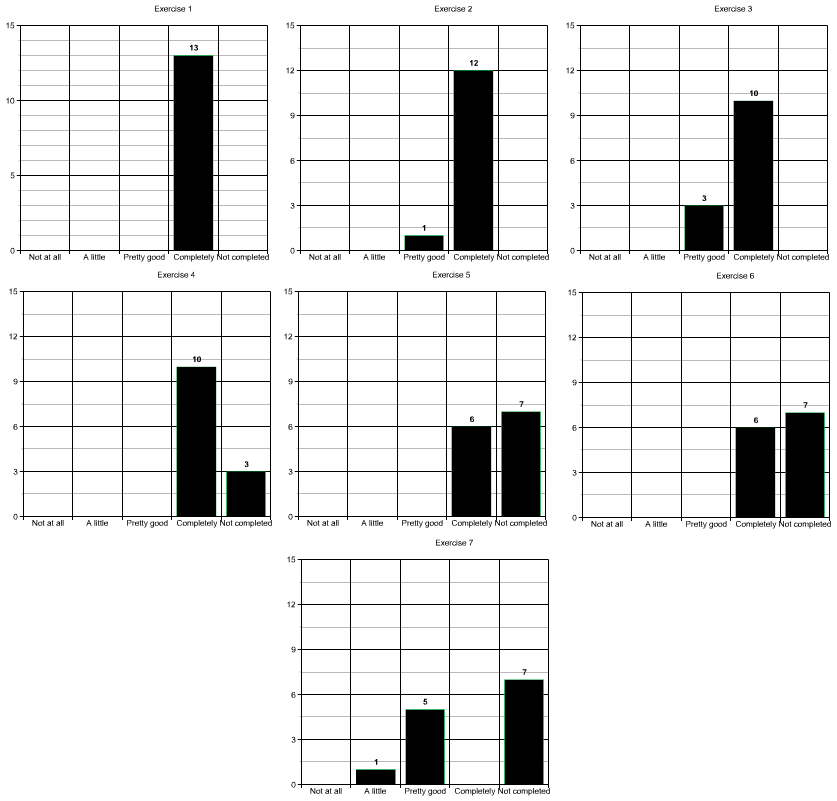
\includegraphics[width=0.75\textwidth]{feedback_form_q3}
	\caption[Results from feedback form question 3]{Results per exercise from question 3 of the feedback form (Appx.~\ref{appx:feedback_form}). The value on the y-axis for all graphs is the number of students who chose that answer. The total number of students was 13.}
	\label{fig:feedback_form_q3}
\end{figure}

\paragraph{Question 4:} Figure~\ref{fig:feedback_form_q45} displays the results from question 4: \emph{``Did you complete any of the challenge exercises?''}. The graph shows that most of the participants chose to complete challenge exercises 1 and 2, half completed exercise 3, and none completed exercises 5 and 7. Comparing this with the results from question 3, we see that all the participants who were able to complete exercises 4 through 7 had also completed challenge exercise 3, and the rest likely did not have time. In any case, the participants seemed motivated for completing the challenge exercises and gaining additional understanding of the concepts presented, but were constrained by time. Challenge exercises 5 and 7 were quite extensive, and would likely have required another 2-hour session.

\paragraph{Question 5:} Figure~\ref{fig:feedback_form_q45} displays the results from question 5, which asked the participants to rate the overall difficulty of the challenge exercises. 1 participant answered too easy, 1 felt that the challenge exercises were of very mixed difficulty, while the remaining found them to be OK. Since these were not meant to be very difficult, and there is likely to be variations in how different participants perceive the difficulty of a given task, this information provides no grounds for changing the difficulty of these exercises.

\begin{figure}[htp]
	\subfloat{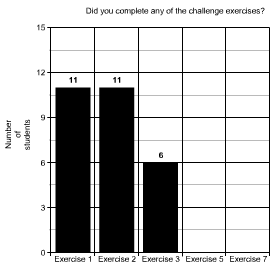
\includegraphics[width=.49\textwidth]{feedback_form_q4}}
	\subfloat{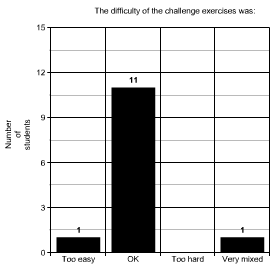
\includegraphics[width=.49\textwidth]{feedback_form_q5}}
	\caption[Results from feedback form questions 4 and 5]{Results from questions 4 (left) and 5 (right) of the feedback form (Appx.~\ref{appx:feedback_form}). The total number of students was 13.}
	\label{fig:feedback_form_q45}
\end{figure}

\paragraph{Question 6:} Since all participants completed at least one of the challenge exercises, there were no answers to this question.

\paragraph{Additional comments:} While only a few of the participants bothered to submit their own thoughts, all of the comments received were positive. It was mentioned that this was a more fun way to learn than regular exercises, and that being able to complete several smaller exercises gave a sense of achievement.

\subsubsection{Observations during the Testing Session}
In addition to the feedback form, I made some observations during the testing session about what the participants struggled with, and discovered some potential problem areas. Most of the observations are a result of the questions the participants asked directly to me.

\paragraph{Technical problems:} Most of the problems the students seemed to have were pure technical, and not related to the learning aspect of the tutorial. Some had trouble installing Eclipse and making it work properly, some had trouble setting up Reactive Blocks within Eclipse. While the tutorial document handed out to each participant contained a brief guide on how to set up and prepare for the tutorial, it appears this guide was not clear or detailed enough for some of the participants, who were unable to complete this process on their own.

\paragraph{Loops and flow breaks:} One of the main purposes of exercise 4 was to understand that loops needed to be split into more than one activity step, for example by the use of a flow break. While I thought this was well explained in the introduction, quite a few participants did not understand this part of the exercise, and had to ask for help. Most seemed to get it after a brief verbal explanation, so it is likely that the introduction part of this particular exercise can be improved.

\paragraph{Decisions and guards:} During the session, I received quite a few questions about how to set guards on decisions in exercise 3. Participants understood that they had to set the decision values somewhere, but they had no idea how. This was not very well explained in the introduction part, and could clearly be improved. This is also reflected by the feedback form results, where some people felt that they lacked some understanding of these concepts.

\paragraph{``Too long, did not read'':} Sometimes, the students asked questions about things that were actually explained in the introduction, and they even seemed to understand it when I just repeated the information they already had. It is hard to know the reason behind this, but one possible explanation is that they did not bother to read the introduction.

\paragraph{Tips section:} Since I had to provide a document instead of the tutorial mode I originally wanted in Reactive Blocks, it was difficult to provide the participants with general tips for solving the exercises in a reasonable way. I had compiled a list of tips at the end of the document, that may have helped the participants with some of the exercises, and even encouraged them to have a look when they encountered trouble. However, they seemed to forget or not know about the tips section, and instead asked me quite a few questions that were more or less directly answered in this section.

\paragraph{Error messages:} When the participants did something wrong, they were generally presented with error messages describing the problem. Very few seemed to understand these error messages however, as they were often presented in the form of Reactive Blocks concepts and terms they were not yet familiar with.

\paragraph{The Reactive Blocks UI:} In addition to questions related to the tutorial, I received a lot of comments about the Reactive Blocks \gls{ui}. Many found the software awkward to use in various ways, and sometimes needed help finding particular elements and functions. Overall, there was a lot of frustration related to things that were outside the scope of the tutorial, such as being able to undo actions in Reactive Blocks.

\subsubsection{Observations after the Testing Session}
During exercise sessions in the following weeks, I was able to make some additional observations based on the questions I received from the students who were working with Reactive Blocks. While I recognized some faces from the testing session, I could not know for sure who had completed the whole tutorial, but some actually made references to it in their questions. The observations made after the testing sessions are mostly based on general impressions, since I did not take note of specific issues. Consequently, this is not very reliable data, but included anyway in order to add some perspective.

\noindent
The most prominent problem the students encountered was that they were poorly prepared for working with Reactive Blocks outside of the tutorial context. They were not comfortable with creating their own local blocks with input/output pins and \glspl{esm}, and still had trouble connecting these to each other in a way that was consistent enough to be accepted by the Reactive Blocks model checker. Often, the problems were directly related to \glspl{esm}, which had not been covered by the tutorial, but sometimes the problems were actually very similar to those presented in the tutorial exercises, just in a different context. The lack of understanding of these concepts is also reflected in the results of the feedback form for exercise 7 (Fig.~\ref{fig:feedback_form_q3}).

\section{Evaluation of the Tutorial}
\label{sec:tutorial_evaluation}
This section provides an evaluation of the Reactive Blocks/\gls{uml} Activities tutorial, with respect to the goals that were set in advance, and the actual usefulness in learning about \gls{uml} modeling. Finally, some suggestions are made as to how the tutorial could be improved.

\subsection{Fulfilled Goals}
\label{sec:tutorial_goal_fulfilled}
Section~\ref{sec:tutorial_goals} lists the goals that were set before creating the Reactive Blocks/\gls{uml} Activities tutorial. This section covers the goals I consider to be fulfilled by the tutorial that was tested.

\paragraph{Interactivity:} For each new concept introduced, users have to become familiar with this concept and some modeling elements by completing an exercise, and possibly an additional challenge exercise. Users become active learners, and have to actually think about the concepts.

\paragraph{Feedback:} Thanks to Reactive Blocks, users are able to execute their models, to see if they behave as intended.

\paragraph{Reasonable Teaching Order:} The teaching order of the concepts and elements was carefully considered to let the users start with the most basic concepts, and then build on these to create more advanced programs. None of the exercises required knowing about concepts that had not been previously introduced.

\paragraph{Context-sensitivity of Information:} The new information required to complete each exercise is presented together with the exercise itself. People also have to retain some information from the previous exercises, but they have the chance to practice and really become familiar with it first.

\paragraph{Multiple Perspectives:} While some of the exercises present a different perspective on some of the concepts through challenge exercises, the contexts are fairly simple. This is a point where the tutorial has room for improvement, so this goal is considered only partially fulfilled.

\paragraph{Difficulty and Challenges:} During the user test, most of the users were able to complete the tutorial exercises. While there were some problems in understanding a few concepts, most of the problems encountered were of a more technical nature, and related to the use of Reactive Blocks. Additional challenge exercises were also present.

\subsection{Not Fulfilled Goals}
Unfortunately, not all of the goals listed in Sect.~\ref{sec:tutorial_goals} were fulfilled. Below are the goals I consider to \textbf{not} be fulfilled by the tutorial that was tested.

\paragraph{Help-on-demand:} I was not able to offer any help-on-demand within the context of the tutorial. Whenever users needed more information, they had to visit the official Reactive Blocks documentation online, or ask an instructor for help.

\paragraph{Visual Mapping of UI Elements:} Since I was unable to make changes to the Reactive Blocks environment, it was difficult to communicate to users how to properly work with the \gls{ui}. During the testing sessions, some participants had trouble finding certain elements.

\paragraph{Freedom:} This goal was also not fulfilled because I was not able to make changes to the Reactive Blocks environment, and thus could not create a proper tutorial mode. However, some of the exercises could be solved in more than one way, giving users some freedom in how to think about the exercises.

\paragraph{Focus on UML Activities:} Also because of a lack of tutorial mode in Reactive Blocks, the tutorial had to teach the users quite a few Reactive Bocks -specific skills for them to be able to work with it.

\paragraph{Avoid Irrelevant Complexities:} No tutorial mode meant no abstraction of tasks like \emph{build and run}, users instead had to learn to do these things manually. Additionally, users were frequently presented with error messages they did not understand, because they had not yet learned enough about Reactive Blocks.

\paragraph{Everything in One Place:} The lack of a tutorial mode forced me to distribute the tutorial over more than one platform. The exercises were completed within Reactive Blocks, but introductions and tasks were presented in a separate document. Additionally, users had to use online documentation to find additional information about a subject.

\subsection{Notes on the Quality of the Tutorial}
\label{sec:tutorial_quality}
Despite not fulfilling all the goals that were set in advance, the tutorial still has some value. Based on the results from the user test, we attempt to get an impression of the actual \emph{quality} of the tutorial. With quality, we consider the tutorial's ability to teach the various concepts and aspects of \gls{uml} Activities, its ability to motivate the users into wanting to learn, and the tutorial's overall usability. A tutorial with a low degree of usability is likely to waste some the users' time on irrelevant troubles.

\subsubsection{Ability to Teach Concepts}
Judging by the results of the user test feedback form, comments received from the participants, and observations of the participants' subsequent work with Reactive Blocks, it seems that this tutorial does a fairly good job of teaching the concepts of \gls{uml} Activities to the target audience. The students appeared to mostly understand the concepts of activity steps and control tokens, as well as how the various model elements worked. They were less equipped to deal with problems related to \glspl{esm} and more advanced modularization, but this was mostly outside the scope of the tutorial. Since I was unable to conduct a comparative study of this tutorial, we can not measure its usefulness for teaching against other similar tutorials.

\subsubsection{Motivating Users}
In the comment section of the feedback form, some of the test participants suggested that the tutorial was a fun way to learn about \gls{uml} Activities and Reactive Blocks, as well as mentioning that completing several smaller exercises gave a sense of achievement after each one. This indicates that the tutorial gives the users some kind of motivation for exploring the topic. Again, it is difficult to compare with other approaches without additional data, but I find it unlikely that a group of students would have classified simply reading through documentation as a \emph{fun way} to learn.

\subsubsection{Usability}
The usability of the tutorial was severely hamstrung by the fact that I could not create a separate tutorial mode in Reactive Blocks. Most of the tutorial resources had to be provided outside the context of Reactive Blocks, which meant the tutorial offered less direct help, and users had to go through a lot of extra effort to find additional information. Users received error messages they could not understand, and even the provided information was in some cases insufficient for users to be able to efficiently complete the tutorial. A prime example is with decisions; many test participants spent a lot more time than they should have trying to figure out how to set guards on branches. With these points in mind, I consider usability to be the tutorial's weakest point. It is possible that in a larger user group, some of these usability issues could prevent a number of users from completing the tutorial without instructor help, or cause them to become too frustrated and lose motivation.

\subsection{Suggestions for Improvement}
\label{sec:tutorial_improvement}
After the tutorial has been tested with a small group of relevant users, some issues have been discovered and briefly discussed. This section suggests how the tutorial can be improved to account for these issues, and thus hopefully provide a better learning experience. 

\begin{itemize}
	\item Have a complete and immersive tutorial mode. This mode should provide the user with the information needed, both introductions as well has help-on-demand and tips, inside the application and in-context, and additionally abstract away processes like choosing Java platform and managing generated code. It should also ideally provide error messages that are better suited to the user's level of experience, and either hide elements that are \emph{less} or highlight elements that are \emph{more} relevant.
	\item In addition to the tutorial mode, the usability of the Reactive Blocks \gls{ui} has some room for improvement, especially for novice users. Making elements available through buttons instead of menus and allowing \emph{undo}-actions are some of the issues that require attention. Improving Reactive Blocks is a little outside our scope, but a better environment is likely to improve the tutorial experience.
	\item The introduction for decisions should be improved to properly explain how guards are set on branches.
	\item Supplement the introductions with animations that illustrate some of the more subtle aspects of \gls{uml} Activities in Reactive Blocks, such as tokens not being able to pass through a given node more than once in each activity step.
	\item If the tutorial will be used to teach users not only about \gls{uml} Activities, but how to work with Reactive Blocks, some additional steps should be created to better prepare users for the real environment. These steps should for example teach users more about different types of blocks, \glspl{esm}, and how to interpret error messages.
\end{itemize}



\cleardoublepage
\chapter{A Tutorial Game: First Iteration}
\label{ch:tutorial_game}

\section{Motivation}
\label{sec:game_motivation}


\section{Concept}
\label{sec:game_concept}


\section{Implementation}
\label{sec:game_implementation}


\section{User Testing and Feedback}
\label{sec:game_testing}
\cleardoublepage
\chapter{Discussion and Conclusion}
\label{ch:discussion}
The work of this thesis has been focused around creating a better environment for learning about software modeling languages, more specifically focusing on \gls{uml} activities within the context of the \emph{Reactive Blocks} modeling tool. Inspired primarily by methods used to teach players how to play video games, two different learning environments were explored.

\section{The Tutorial}
\label{sec:discussion_tutorial}
The first teaching method explored was the \emph{tutorial}, a concept widely used to teach various topics by offering interactive introductions, often with exercises. This approach to teaching is also used in many video games, where players are exposed to a tutorial that teaches them the basics of the game before they are allowed to explore the game on their own. The design, implementation, testing, and evaluation of the tutorial is covered in Ch.~\ref{ch:reactive_blocks_tutorial}.

\noindent
When creating the tutorial, various learning practices were taken into consideration. These were a mixture of good practices for video game tutorials and other types of tutorials, from both formal and informal sources. A summary of these is provided in Sect.~\ref{sec:good_practices_tutorials}.

\noindent
A few iterations of going through \gls{uml} activity concepts and figuring out their interdependencies, finding the least amount of information required to describe them accurately, and designing suitable exercises for understanding their semantics, resulted in a seven-step tutorial. Each step gave a short introduction of one or more concepts, and challenged learners with an exercise to solve using these concepts. The tutorial and its seven steps is described in more detail in Sect.~\ref{sec:tutorial_design}.

\noindent
Unfortunately, not all of these practices were feasible to implement within the given frame, particularly because of the constrains provided by the proprietary Reactive Blocks modeling environment. This meant some of the goals that had initially been set for the tutorial had to be forgone, and some adjustments had to be made to the tutorial design. The most prominent change was that all concept and task information had to be provided outside the modeling environment, in a supplementary document. Sections~\ref{sec:tutorial_goals_fulfilled} and~\ref{sec:tutorial_goals_not_fulfilled} provide a more detailed overview of the extent to which each goal was fulfilled by the tutorial design and implementation.

\noindent
In order to uncover any major flaws or issues with the tutorial, and additionally get an impression of its teaching potential, a user test with a small number of test subjects was conducted. The testing session revealed a number of issues that required some additional consideration, and the main bulk of these were related, directly or indirectly, to the use of Reactive Blocks as the modeling environment. The session also provided some indications that the tutorial could indeed be a very good way of learning about \gls{uml} activities, particularly with respect to providing motivation for learners. The tutorial may not be an adequate tool for learning to use Reactive Blocks however, as follow-up observations of the test subjects revealed that many of them struggled when working with Reactive Blocks, on account of the concepts that were not covered in the tutorial.

\noindent
Although I was unable to implement and test several of the tutorial design principles, the tutorial served as a good starting point for establishing a teaching order for concepts in \gls{uml} activities, and figuring out how much information users need in order to solve certain types of exercises related to each concept. These results laid the foundation for the \emph{Reactive Blocks game}, which was the second teaching method explored.

\section{The Game}
\label{sec:discussion_game}
The second teaching method explored in this thesis was to teach \gls{uml} activity concepts inside a game. Learning games are becoming very popular in many levels of education because they offer a more immersive and interactive learning experience, among other things. Teaching \gls{uml} activities with a game gave more potential for utilizing game strategies for introducing and teaching new concepts, such as giving learners a sense of \emph{empowerment} and \emph{identity}. The design, implementation, testing, and evaluation of the learning game is covered in Ch.~\ref{ch:tutorial_game}.

\noindent
Like with the tutorial, the learning game is based on a set of principles for designing this type of game, and these are summarized in Sect.~\ref{sec:good_practices_games}. Additionally, the game would have a lot in common with a tutorial, so consideration was made with respect to the principles for good tutorials, and the lessons learned from the design and testing of the tutorial in Ch.~\ref{ch:reactive_blocks_tutorial}.

\noindent
The design and implementation process resulted in a first prototype version of a game with 5 levels, covering only part of the seven steps from the tutorial. The game was meant to have more levels, but we wanted to conduct a usability study in order to discover any serious issues as early as possible. The concept of the game is a two-dimensional world, where the player controls a character, performing various tasks. The character is controlled entirely through \gls{uml} activity/Reactive Blocks models, which the player has to set up prior to launching the game level. Each level also has an introduction part, similar to the introductions given with the tutorial, but more extensive and with additional resources. The complete design and implementation of the game is covered in Sections~\ref{sec:game_design} and~\ref{sec:game_implementation}.

\noindent
While the game format allowed consideration and implementation of some additional ``good'' practices, there were still issues that were difficult to deal with because of the Reactive Blocks modeling environment. A usability test with three test subjects revealed that all three, who were novice users, had difficulties with correctly understanding and using a number of \gls{ui} processes and elements in Reactive Blocks. This was despite the fact that some additional \gls{ui} help had been added to the introduction part of the game, as a result of some of the same issues appearing in the tutorial test. Apart from those related to Reactive Blocks, the usability test revealed only minor \gls{ui} issues that could be taken into consideration for the next version of the prototype.

\noindent
In addition to usability-related results, the testing sessions also revealed that the test subjects gained a lower understanding of the concepts presented than desired. Some hints of potential misconceptions were also observed. This could likely mean that 5 levels is not sufficient to really learn these concepts, and that more practice is required. If this is the case, it can be solved by adding additional levels and challenges, for the players to practice their skills and knowledge more, and with different perspectives. In any case, more testing is needed to properly verify and understand the issue, preferably on a more complete version of the game.

\noindent
On a brighter note, all three subjects stated that they enjoyed the game as a tool for learning about \gls{uml} activities and Reactive Blocks, and would likely prefer it over other ways of learning. However, more than three opinions are likely needed in order to verify a real interest in this type of learning resource. It also remains to be seen whether a game like this will instill deep learning in players, but research supports that this is the case for well-designed educational games (see Sect.~\ref{sec:game_based_learning}).

\noindent
The game is still in a relatively early stage, but the results so far are encouraging. Further development of the game will however not continue within the scope of this thesis, because of time constraints.


\section{Concluding Remarks}
\label{sec:concluding_remarks}
The work of this thesis has been about exploring the use of game-related learning principles and strategies for teaching software modeling with \gls{uml} activities. Two different teaching approaches were explored:  the first approach simply incorporated many of the learning principles in a stepwise modeling tutorial, and the second approach involved designing a game with levels teaching the same steps, but in a more immersive environment.

\noindent
Some minor tests of the two approaches were conducted, yielding indicative but interesting results. Both approaches were found to be flawed in some ways, but they also showed great potential for teaching the concepts in question to the target audience in an interesting and motivating way. It is however difficult to draw any conclusions about how the two approaches would measure up against other learning resources for the same concepts, without data from comparative studies.

\noindent
It is also worth noting that with regard to established theoretical usability and learning principles, both approaches measure up quite well by \emph{design}, despite the \emph{implementations} lacking some important features. Whether implementing all of these features will actually be beneficial to the learning experience or not is however a little uncertain, as users have been known to behave unpredictably~\cite{andersen:tutorials_impact}.

\noindent
In the end, there is no reason to believe that learning strategies from games will \emph{not} be appropriate also for learning modeling languages, as there have been no results indicating this. At the same time, there is not enough ground in this thesis alone to conclude that they \emph{definitely will be} appropriate either. There are however several other research efforts endorsing this approach for teaching programming, which is a very closely related topic.

\noindent
The conclusion to be drawn from this thesis is the following: using learning strategies from games to teach modeling languages is definitely worth exploring, but designing and implementing a good learning environment is not trivial, and requires a considerable amount of work and effort. Hopefully, the work and examples provided here can serve as a starting point for others.

\clearpage

\section{Future Work}
\label{sec:future_work}
As the final part of this thesis, some suggestions for future work are included. There are several possible paths to take, and some are described in the following sections.

\subsection{Complete Game}
The most prominent path to take would be to continue development of the Reactive Blocks game, improving on the prototype and moving closer to a ``finished'' game. The current prototype is a little lacking in content, in addition to needing some minor fixing. There is also great potential for improving the modeling environment, particularly in order to improve usability. Section.~\ref{sec:game_improvement} contains some more concrete suggestions on how to continue the development of the game. 

\subsection{Comparative Studies}
The weakest part of this thesis is likely that I was unable to perform proper comparative studies, pitting the \emph{Reactive Blocks game} against other similar learning resources in order to measure factors like player engagement and levels of understanding. This was not feasible because of constraints on time and resources. Comparative studies would however have been prudent in this context, and should thus be the second priority for any future work (after fixing the simpler issues and adding more content to the game).

\noindent
More specifically, the game can be studied in comparison to the tutorial in Ch.~\ref{ch:reactive_blocks_tutorial}, any of the existing tutorials mentioned in Sect.~\ref{sec:existing_tutorials}, or the lazier approach of just letting learners dig through documentation.

\subsection{Other Modeling Languages}
This thesis has been focused around teaching \gls{uml} activities, more specifically in the context of Reactive Blocks, using teaching principles and strategies from games. It could also be interesting to use the same approach with other modeling languages, such as \gls{uml} state machines, sequence diagrams, flowcharts, or even class diagrams. These will likely provide different challenges with respect to game and exercise design, but allow use of the same teaching principles.
\cleardoublepage

\renewcommand*{\bibname}{References}
\bibliographystyle{alpha}
\bibliography{main}

%% Uncomment the following if you have any appendix
\appendix
\addtocontents{toc}{%
 \protect\vspace{1em}% 
 \protect\noindent \bfseries \appendixtocname\protect\par
 \protect\vspace{-.5em}%
}
\renewcommand{\chaptername}{\appendixname}
%% include below possible appendices (chapters)
\begin{appendices}

\chapter{UML Activities Tutorial}
\label{appx:tutorial}
The following pages contain the complete document for the Reactive Blocks \gls{uml} Activities tutorial described in Ch.~\ref{ch:reactive_blocks_tutorial}.
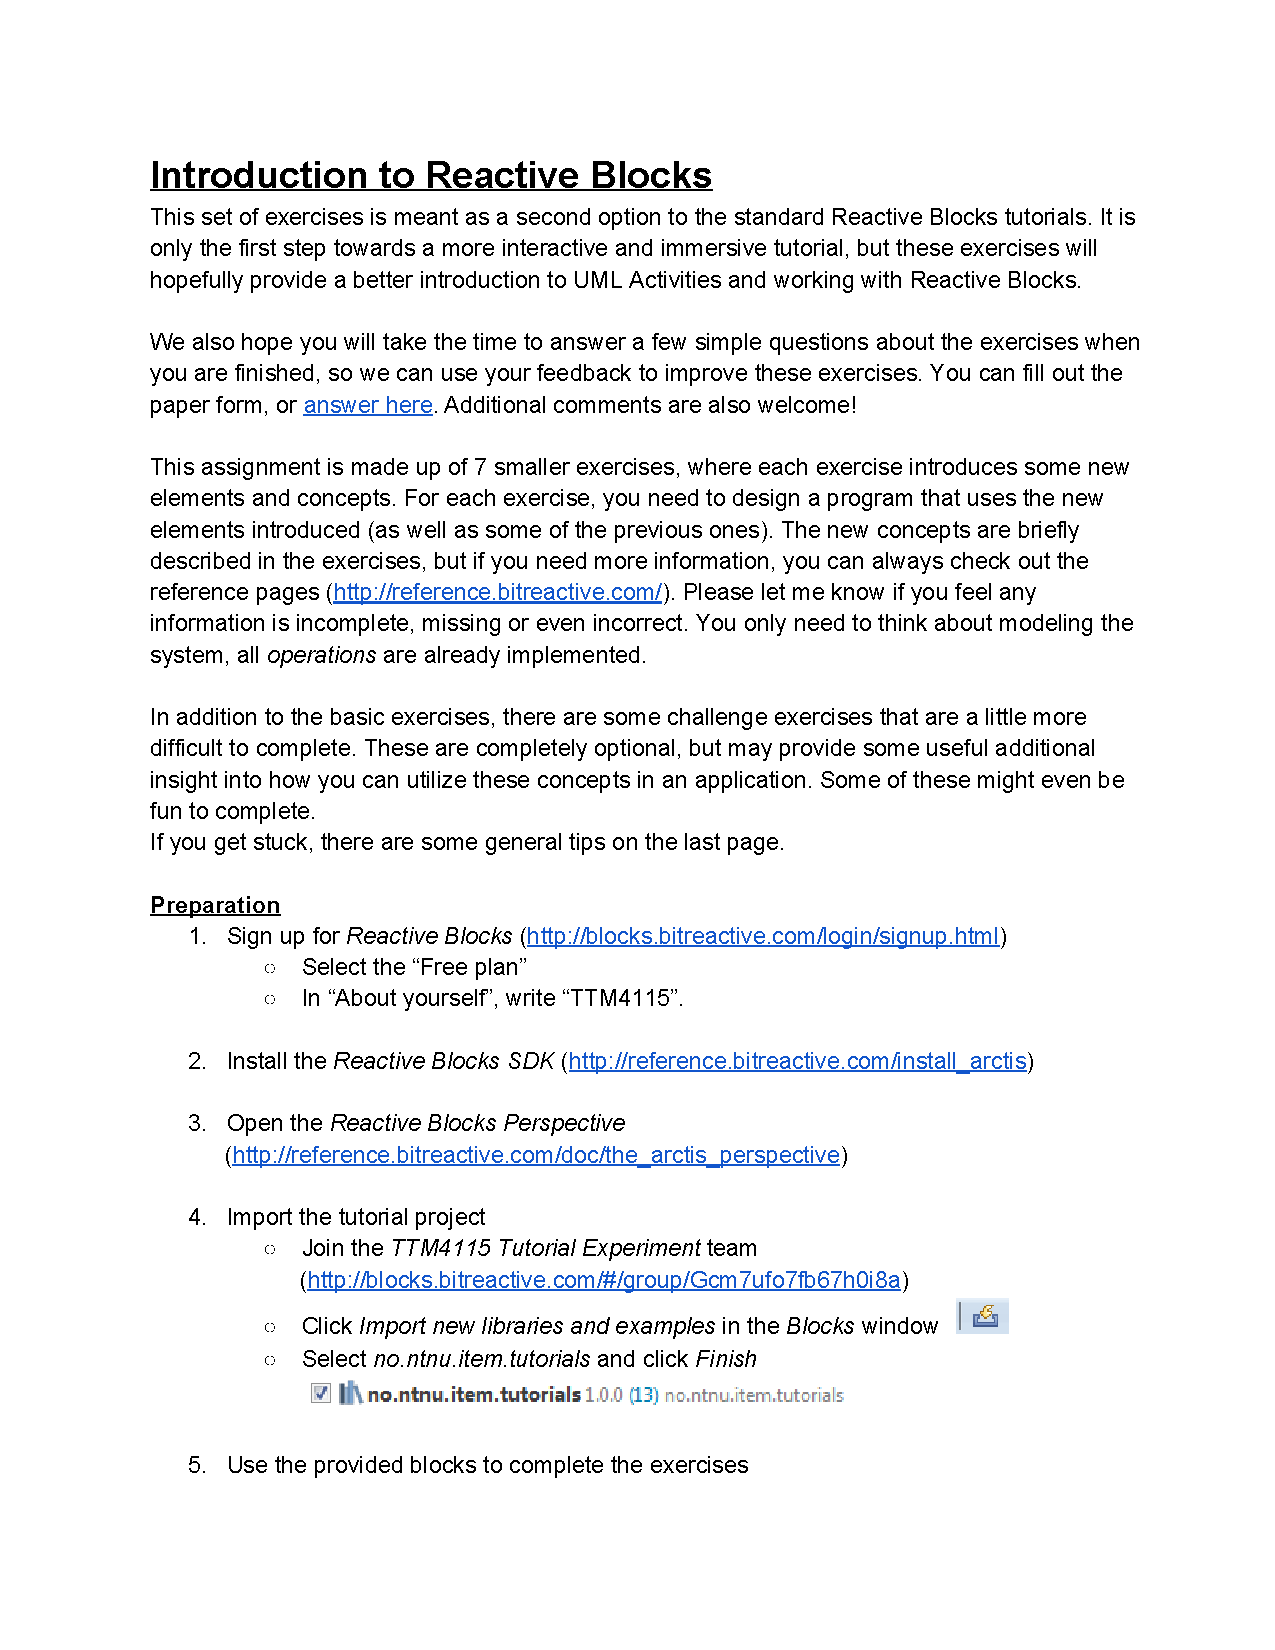
\includepdf[pages={-}]{tutorial_exercises.pdf}

\chapter{Tutorial Feedback Form}
\label{appx:feedback_form}

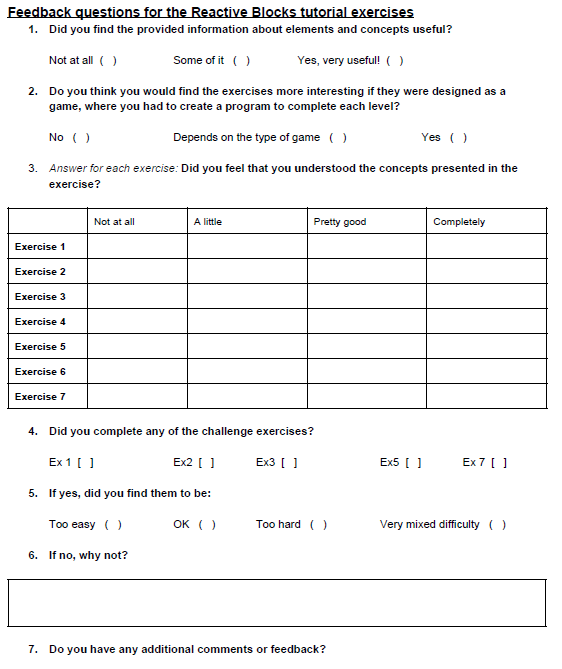
\includegraphics[scale=0.75]{tutorial_feedback}

\chapter{Tutorial User Test Data}
\label{appx:tutorial_test_data}
This section contains all the data gathered with the feedback forms (Appx.~\ref{appx:feedback_form}) in the user test for the Reactive Blocks/\gls{uml} Activities tutorial (Ch.~\ref{ch:reactive_blocks_tutorial}).

\begin{figure}[htp]
	\centering
	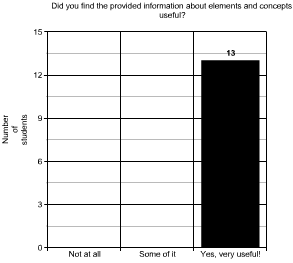
\includegraphics[scale=0.80]{feedback_form_q1}
	\caption[Results from feedback form question 1]{Results from question 1 of the feedback form (Appx.~\ref{appx:feedback_form}). The total number of students was 13.}
	\label{fig:feedback_form_q1}
\end{figure}

\begin{figure}[htp]
	\centering
	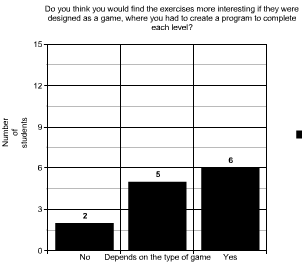
\includegraphics[scale=0.80]{feedback_form_q2}
	\caption[Results from feedback form question 2]{Results from question 2 of the feedback form (Appx.~\ref{appx:feedback_form}). The total number of students was 13.}
	\label{fig:feedback_form_q2}
\end{figure}

\begin{figure}[htp]
	\centering
	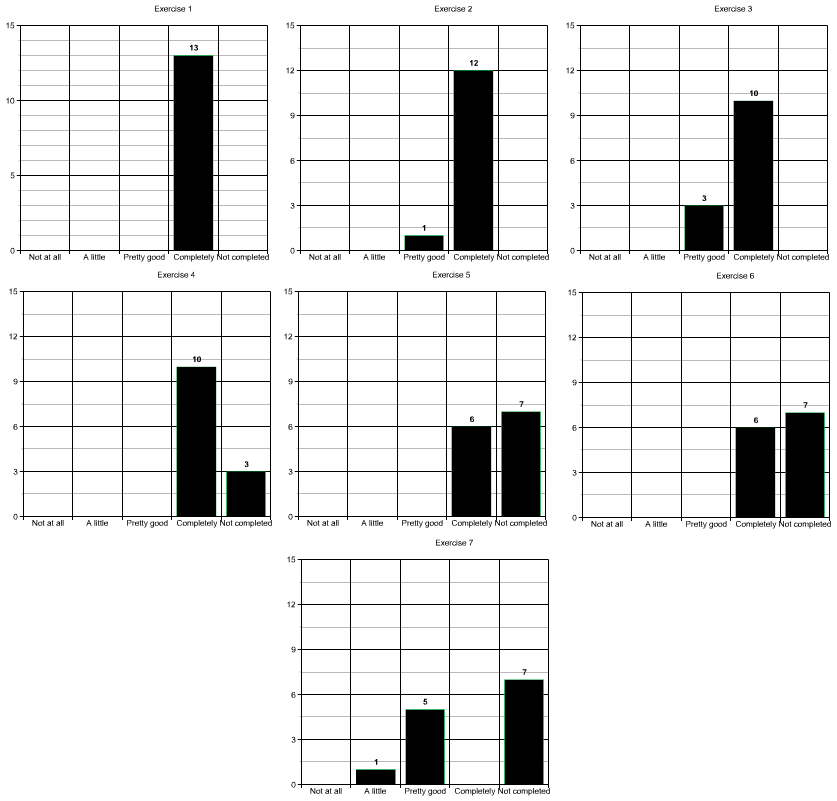
\includegraphics[scale=0.55]{feedback_form_q3}
	\caption[Results from feedback form question 3]{Results per exercise from question 3 of the feedback form (Appx.~\ref{appx:feedback_form}). The value on the y-axis for all graphs is the number of students who chose that answer. The total number of students was 13.}
	\label{fig:feedback_form_q3}
\end{figure}

\begin{figure}[htp]
	\centering
	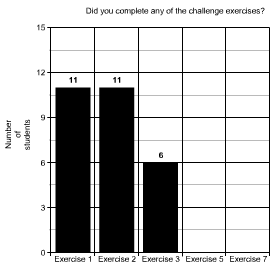
\includegraphics[scale=0.80]{feedback_form_q4}
	\caption[Results from feedback form question 4]{Results from question 4 of the feedback form (Appx.~\ref{appx:feedback_form}). The total number of students was 13.}
	\label{fig:feedback_form_q4}
\end{figure}

\begin{figure}[htp]
	\centering
	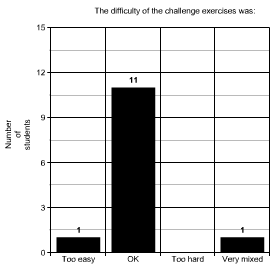
\includegraphics[scale=0.80]{feedback_form_q5}
	\caption[Results from feedback form question 5]{Results from question 5 of the feedback form (Appx.~\ref{appx:feedback_form}). The total number of students was 13.}
	\label{fig:feedback_form_q5}
\end{figure}

\chapter{Feedback Form for the Game Usability Test}
\label{appx:game_feedback_form}

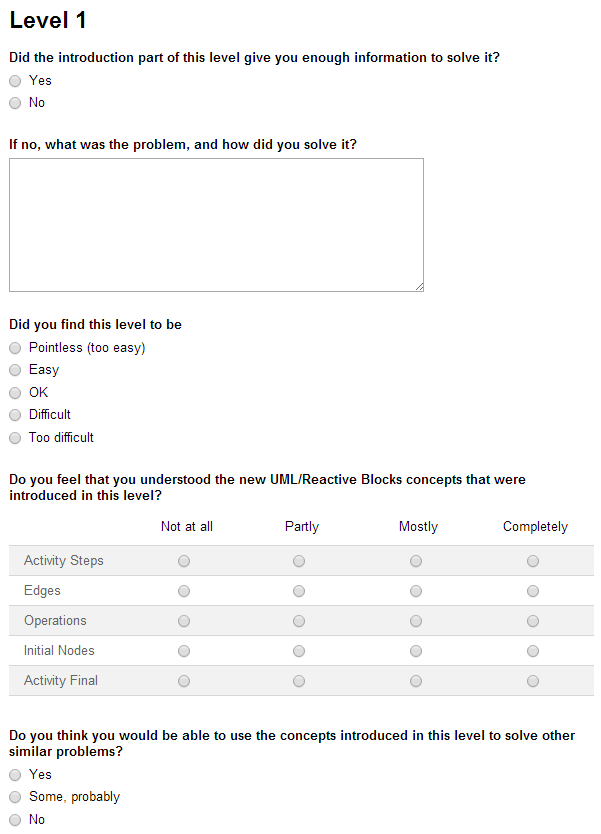
\includegraphics[scale=0.60]{usability_quiz}







\end{appendices}


\end{document} 
